\chapter{Recherche de résonances de spin 0 dans le spectre de masse \ttbar} \label{chap:higgs}

\begin{fmffile}{chapitre8}

Ce chapitre est dédié à la recherche de résonance de spin 0 (\sz) dans le spectre de masse \ttbar. Contrairement à l'analyse présentée dans le \cref{chap:zprime} (analyse \zprime), cette analyse se base sur un modèle particulier. On interprète en effet la résonance de spin 0 comme un boson de Higgs massif se désintégrant exclusivement en \ttbar, comme prédit par exemple par un modèle à deux doublets de Higgs (voir \cref{sec:2hdm}).

La recherche d'une particule de spin 0 comporte plusieurs difficultés, de la génération du signal jusqu'à la stratégie d'analyse. Dans ce chapitre, certaines de ces problématiques sont résolues. Pour d'autres, les résultats sont encore très préliminaires et seule une étude de faisabilité est présentée. Cette recherche se révèle à la fois difficile et prometteuse.

\section{Signaux et bruits de fonds}

La production de particules de spin 0 se désintégrant exclusivement en \ttbar se fait par fusion de gluons, à l'aide d'une boucle de quarks top. Le diagramme de Feynman de cette production est visible sur la \cref{fig:f_signal_alone}. Le couplage $g_{\sz \ttbar}$ de la résonance aux quarks top est défini par
\begin{align*}
  g_{\sz \ttbar} &= \alpha \, i \frac{m_{\Ptop}}{v} + \beta \, \gfive \frac{m_{\Ptop}}{v}
\end{align*}
et comporte deux parties : une scalaire, proportionnelle à $\alpha$, et une pseudo\-/scalaire, proportionnelle à $\beta$. Ainsi, il est possible de générer des particules purement scalaires ($\alpha \neq 0$, $\beta = 0$), purement pseudo\-/scalaires ($\alpha = 0$, $\beta \neq 0$), voire un mélange d'états scalaires - pseudo\-/scalaires.

\begin{figure}[tbp] \centering
\begin{fmfgraph*}(160,70) \fmfkeep{higgs}
      \fmfpen{0.5}
      \fmfleftn{i}{2} \fmfrightn{o}{2}
      \fmf{gluon,tension=1.3}{i1,v1}
      \fmf{gluon,tension=1.3}{i2,v2}
      \fmf{fermion,tension=0.8}{v1,v2,v3}
      \fmf{fermion,tension=0.8}{v3,v1}
      \fmf{dashes,label=\sz,tension=1,label.side=left}{v3,v4}
      \fmf{fermion,tension=0.72}{o1,v4,o2}
      \fmfv{label=\Ptop}{o1}
      \fmfv{label=\APtop}{o2}
      \fmfdot{v3,v4}
\end{fmfgraph*}
\caption{Diagramme de Feynman de la production d'un \sz par fusion de gluons. Seuls les quarks top participent à la boucle de quarks.}
\label{fig:f_signal_alone}
\end{figure}

\medskip

Pour étudier cette production, on ajoute à la simulation Monte-Carlo une nouvelle particule scalaire non-colorée. Dans l'étude présentée dans ce chapitre, deux types de signaux sont générés :
\begin{itemize}
    \item Une résonance purement scalaire, avec un couplage $g_{\sz \ttbar} = i \frac{m_{\Ptop}}{v}$.
    \item Une résonance purement pseudo\-/scalaire, avec un couplage $g_{\sz \ttbar} = \gfive \frac{m_{\Ptop}}{v}$.
\end{itemize}

Il est intéressant de placer cette étude dans le contexte du modèle 2HDM \citep{Lee:1973iz,PhysRevD.15.1958,PhysRevD.18.2574}. En se plaçant dans le cas où le boson de Higgs observé au LHC serait le boson scalaire léger \Phz du modèle, on interprète notre nouvelle particule comme les bosons scalaires massifs \PHz (scalaire) ou \PAz (pseudo\-/scalaire). Dans certains modèles, comme par exemple le MSSM, la désintégration des bosons \PHz / \PAz en \ttbar est dominante dans certaines régions de l'espace des paramètres, notamment à bas $\tan(\beta)$. Ces régions ne sont pas encore exclues par les mesures disponibles, et la recherche de signaux en \ttbar est donc la seule façon de les contraindre.

Lors de la génération du signal, le rapport d'embranchement en \ttbar est fixé à \SI{100}{\percent}, et la section efficace ainsi que la largeur de la résonance sont fixées par la masse et le type de la résonance (voir \cref{eq:sigma_scalar,eq:sigma_pscalar}). Plusieurs masses sont générées, allant de \SI{400}{\GeV} à \SI{800}{\GeV} par pas de \SI{100}{\GeV}.

\bigskip

Cette analyse se concentre sur les désintégrations semi\-/leptoniques des paires \ttbar. Les bruits de fonds considérés sont résumés dans le \cref{tab:backgrounds_higgs}.

\begin{eq}[p!]
    \begin{align*}
      \hat{s} &= \mtt^2 \; , \qquad \beta = \sqrt{ 1 - \frac{4 \mt^2}{\hat{s}} }, \qquad y_t = \ln\left( \frac{1 + \beta}{1 - \beta} \right), \qquad \Gamma_{\sz} = \frac{3 G_F \mt^2 \hat{s}\beta^3}{4 \pi \msz \sqrt{2}} \\
      \begin{split}
          \sigma(\hat{s}) &= \overbrace{\frac{ 3 \alpha_s^2 G_F^2 m_t^6 \beta^3 }{ 2048 \pi^3 } \frac{ 16 + 8 \beta^2\left(\pi^2 -y_t^2\right) + \beta^4\left(y_t^2 + \pi^2\right)^2 }{ \left(\hat{s} - m_{\sz}^2\right)^2 + m_{\sz}^2\Gamma_{\sz}^2 }}^{\text{signal scalaire}} \\
          &- \underbrace{\frac{ \alpha_s^2 G_F m_t^4 \beta^2 }{ 32 \pi \sqrt{2} \hat{s} } y_t \frac{ \left(\hat{s} - m_{\sz}^2\right) \left(4 + \beta^2 \left(\pi^2 - y_t^2\right)\right) + 2 \pi \beta^2 m_{\sz} \Gamma_{\sz} y_t }{ \left(\hat{s} - m_{\sz}^2\right)^2 + m_{\sz}^2\Gamma_{\sz}^2 }}_{\text{interférences}} \\
          &+ \sigma_\text{QCD}(\hat{s})
      \end{split}
    \end{align*}
    \caption{Section efficace de production pour un \sz scalaire, adaptée de \citep{Dicus:1994bm}.}
    \label{eq:sigma_scalar}
\end{eq}
\begin{eq}
    \begin{align*}
      \hat{s} &= \mtt^2 \, , \qquad \beta = \sqrt{ 1 - \frac{4 \mt^2}{\hat{s}} }, \qquad y_t = \ln\left( \frac{1 + \beta}{1 - \beta} \right), \qquad \Gamma_{\sz} = \frac{3 G_F \mt^2 \hat{s}\beta}{4 \pi \msz \sqrt{2}} \\
      \begin{split}
          \sigma(\hat{s}) &= \overbrace{\frac{ 3 \alpha_s^2 G_F^2 m_t^6 \beta }{ 2048 \pi^3 } \frac{ \left(y_t^2 + \pi^2\right)^2 }{ \left(\hat{s} - m_{\sz}^2\right)^2 + m_{\sz}^2\Gamma_{\sz}^2 }}^{\text{signal pseudo-scalaire}} \\
                       &- \underbrace{\frac{ \alpha_s^2 G_F m_t^4 }{ 32 \pi \sqrt{2} \hat{s} } y_t \frac{ \left(\hat{s} - m_{\sz}^2\right) \left(\pi^2 - y_t^2\right) + 2 \pi m_{\sz} \Gamma_{\sz} y_t }{ \left(\hat{s} - m_{\sz}^2\right)^2 + m_{\sz}^2\Gamma_{\sz}^2 }}_{\text{interférences}} \\
                       &+ \sigma_\text{QCD}(\hat{s})
      \end{split}
    \end{align*}
    \caption{Section efficace de production pour un \sz pseudo\-/scalaire, adaptée de \citep{Dicus:1994bm}.}
    \label{eq:sigma_pscalar}
\end{eq}

\begin{table} \centering
  \begin{tabular}{@{}ccc@{}} \toprule
    Processus & Section efficace (\si{\pb}) & Luminosité équivalente (\si{\invfb}) \\ \midrule
    \ttbar & \num{245.8} (NNLO) & \num{84.3} \\
    \PW + jets & \num{37509} (NNLO) & \num{1.5} \\
    \PZ + jets & \num{3504} (NNLO) & \num{8.7} \\
    Top célibataire (voie s) & \num{5,6} (NNLO appr.) & \num{72.0} \\
    Top célibataire (voie t) & \num{87,1} (NNLO appr.) & \num{65.4} \\
    Top célibataire (voie t\PW) & \num{22.4} (NNLO appr.) & \num{44.3} \\
    Di-bosons & \num{97,2} (NLO) & \num{30.7} \\
    \bottomrule
  \end{tabular}
  \caption{Section efficace et luminosité équivalente pour chacun des bruits de fond considérés.}
  \label{tab:backgrounds_higgs}
\end{table}

% \bigskip

% Afin de reproduire correctement les conditions de \pu des données, les événements dans la simulation sont pondérés de telle sorte que la distribution du nombre d'interactions par croisement de faisceau soit identique dans les données et la simulation.

\subsection{Génération du signal}

Les états initiaux et finaux de la production de \sz sont identiques à ceux du mode de production dominant de quarks top Modèle Standard au LHC. Comme évoqué brièvement \cref{sec:2hdm}, la production de \sz va interférer avec celle du Modèle Standard, ne conduisant pas simplement à un pic dans la masse invariante dans le spectre \mtt, mais à une structure plus compliquée de type pic - trou. Les \cref{eq:sigma_scalar,eq:sigma_pscalar} (adaptées de \citep{Dicus:1994bm}) présentent respectivement les sections efficaces théoriques pour un scalaire et un pseudo-scalaire dans le modèle 2HDM. La somme des termes de signal et d'interférence est représentée sur la \cref{fig:theo_sigma}, pour différents points de masse. La présence d'une telle particule donne lieu à deux effets localisés : un excès et un déficit d'événements par rapport à la prédiction du Modèle Standard. L'effet des interférences est non négligeable, le déficit étant parfois plus important que l'excès. La contribution du signal et de l'interférence à l'excès et au déficit est présentée sur la \cref{fig:signal_interference}.

\begin{figure}[tbp] \centering
    \subcaptionbox{Scalaire}[0.48\textwidth]{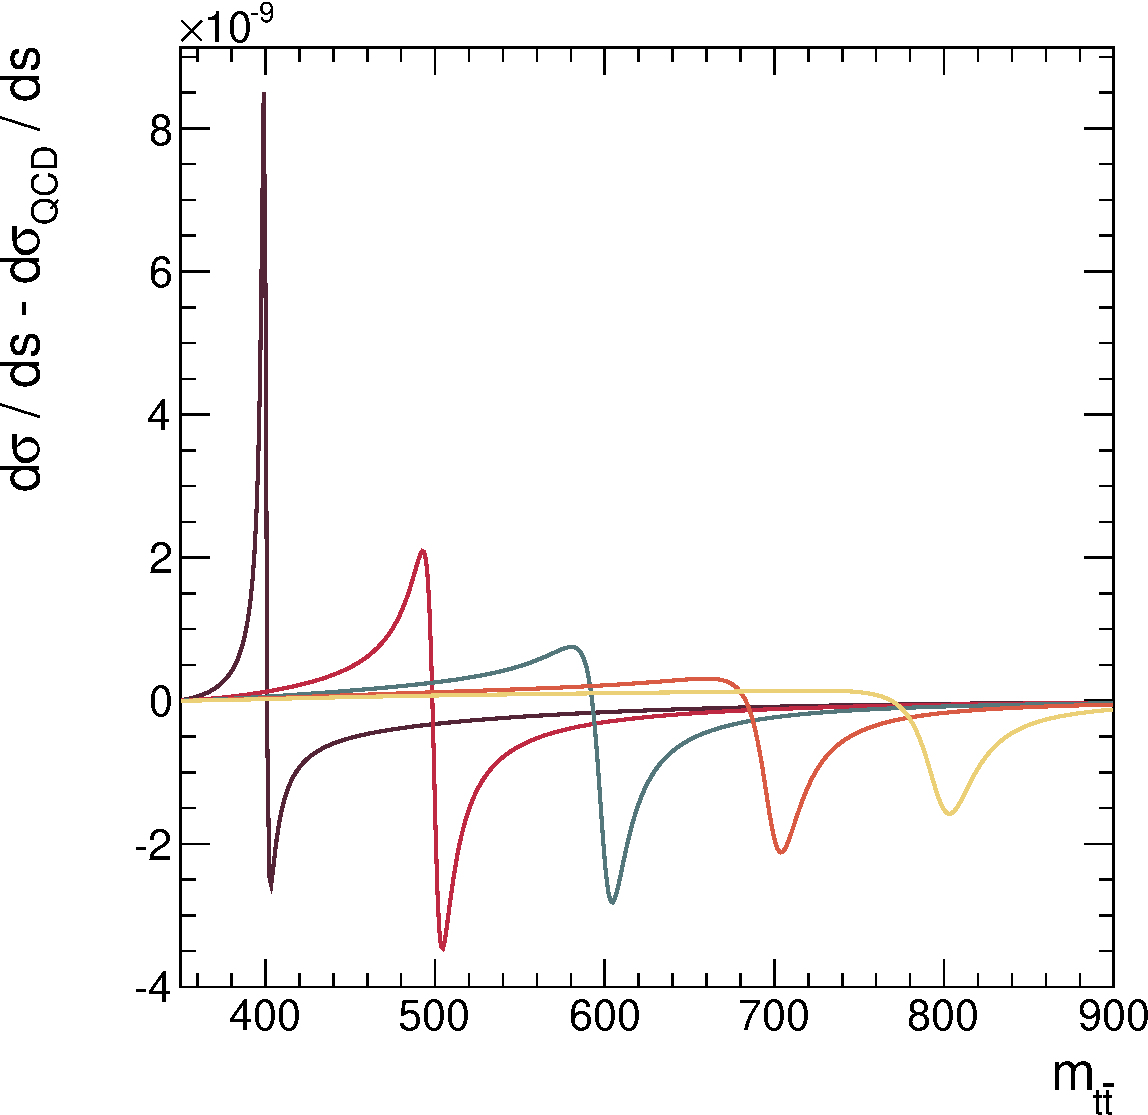
\includegraphics[width=0.48\textwidth,angle=-90,origin=c]{chapitre8/figs/S0/theory_scalar.pdf}} \hfill
    \subcaptionbox{Pseudo-scalaire}[0.48\textwidth]{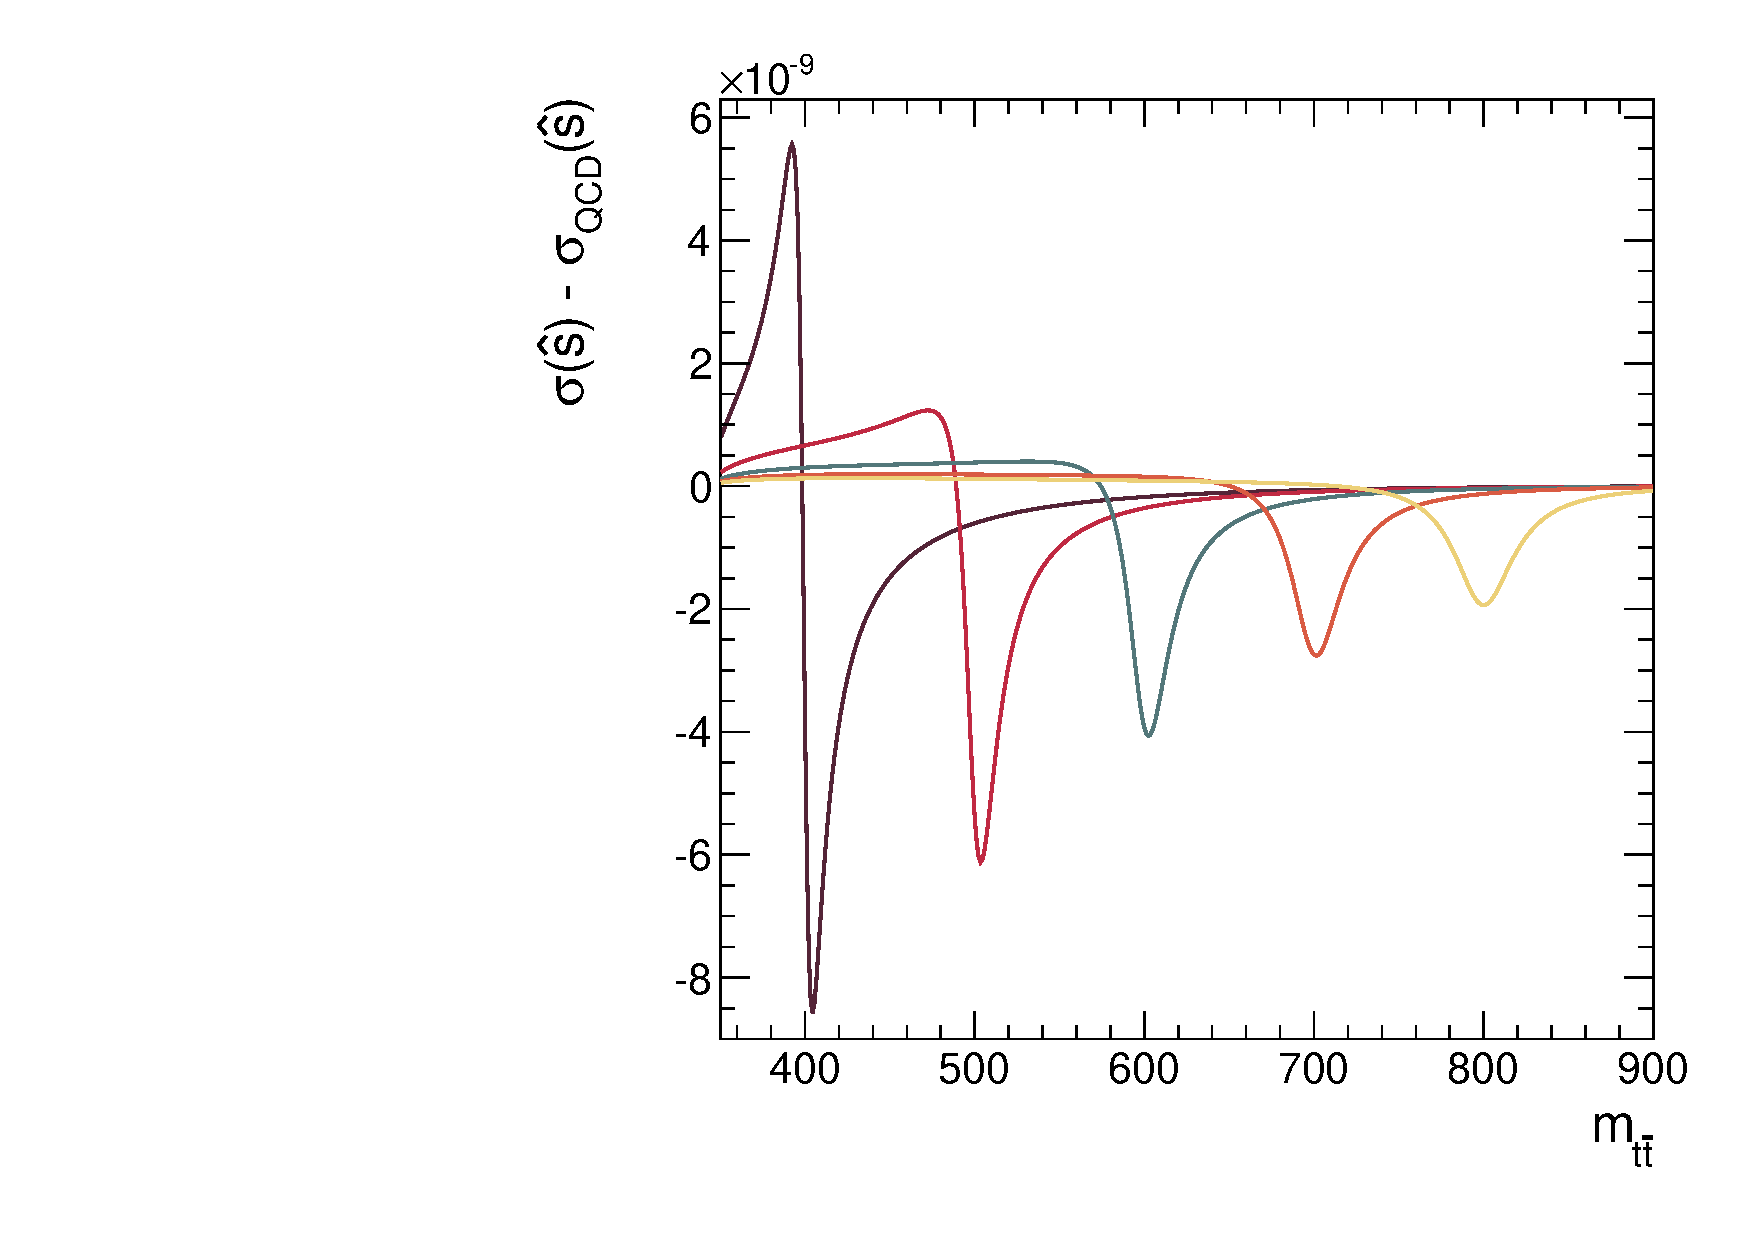
\includegraphics[width=0.48\textwidth,angle=-90,origin=c]{chapitre8/figs/S0/theory_pseudoscalar.pdf}}
    \caption{Section efficace signal + interférences obtenue à l'aide des \cref{eq:sigma_scalar,eq:sigma_pscalar}, pour la désintégration $\sz \rightarrow \ttbar$ en fonction de \mtt, pour différentes masses de signal. Les PDFs des partons ne sont pas incluses dans le calcul. On rappelle que la largeur dépend de la masse de la résonance.}
    \label{fig:theo_sigma}
\end{figure}

\begin{figure}[tbp] \centering
    \subcaptionbox{Scalaire, $\msz = \SI{500}{\GeV}$}[0.48\textwidth]{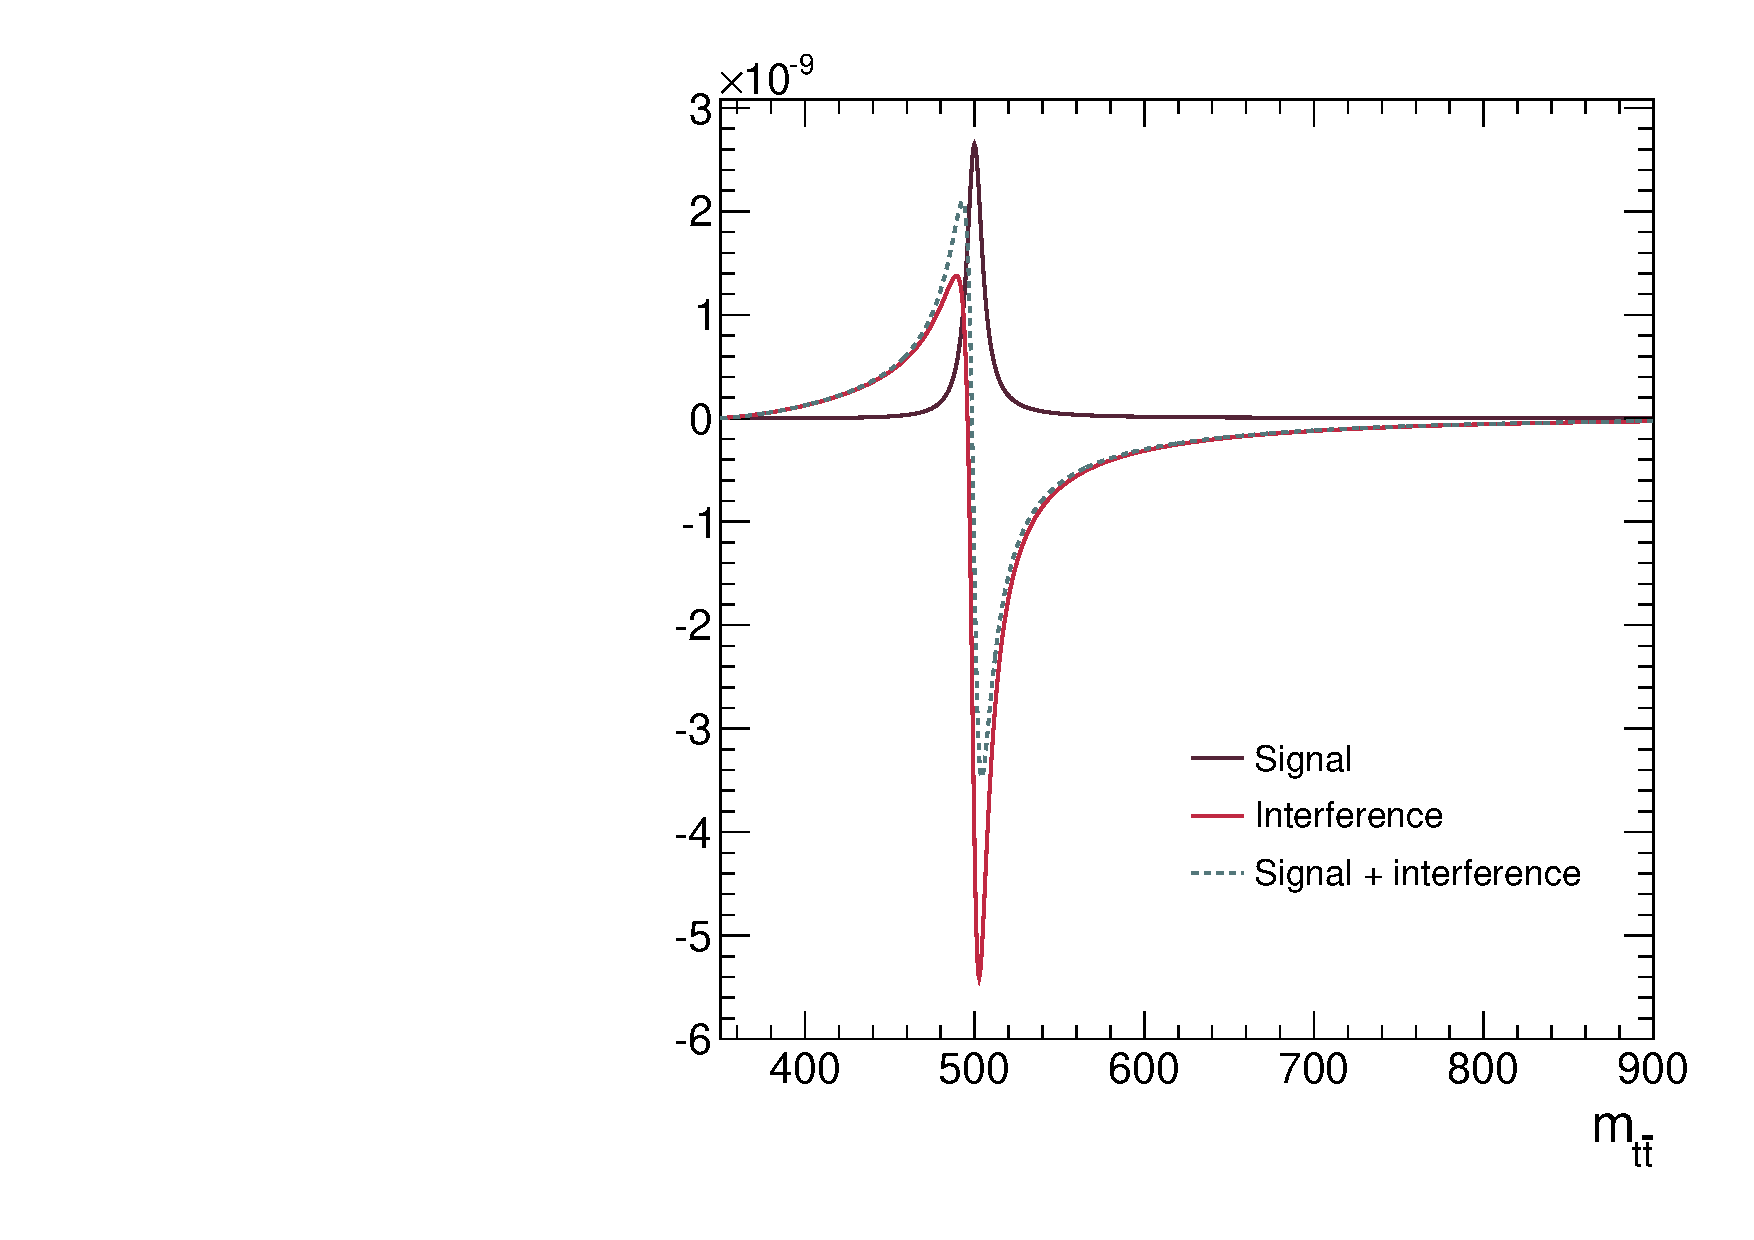
\includegraphics[width=0.48\textwidth,angle=-90,origin=c]{chapitre8/figs/S0/theory_scalar_500_sig_int.pdf}} \hfill
    \subcaptionbox{Pseudo-scalaire, $\msz = \SI{500}{\GeV}$}[0.48\textwidth]{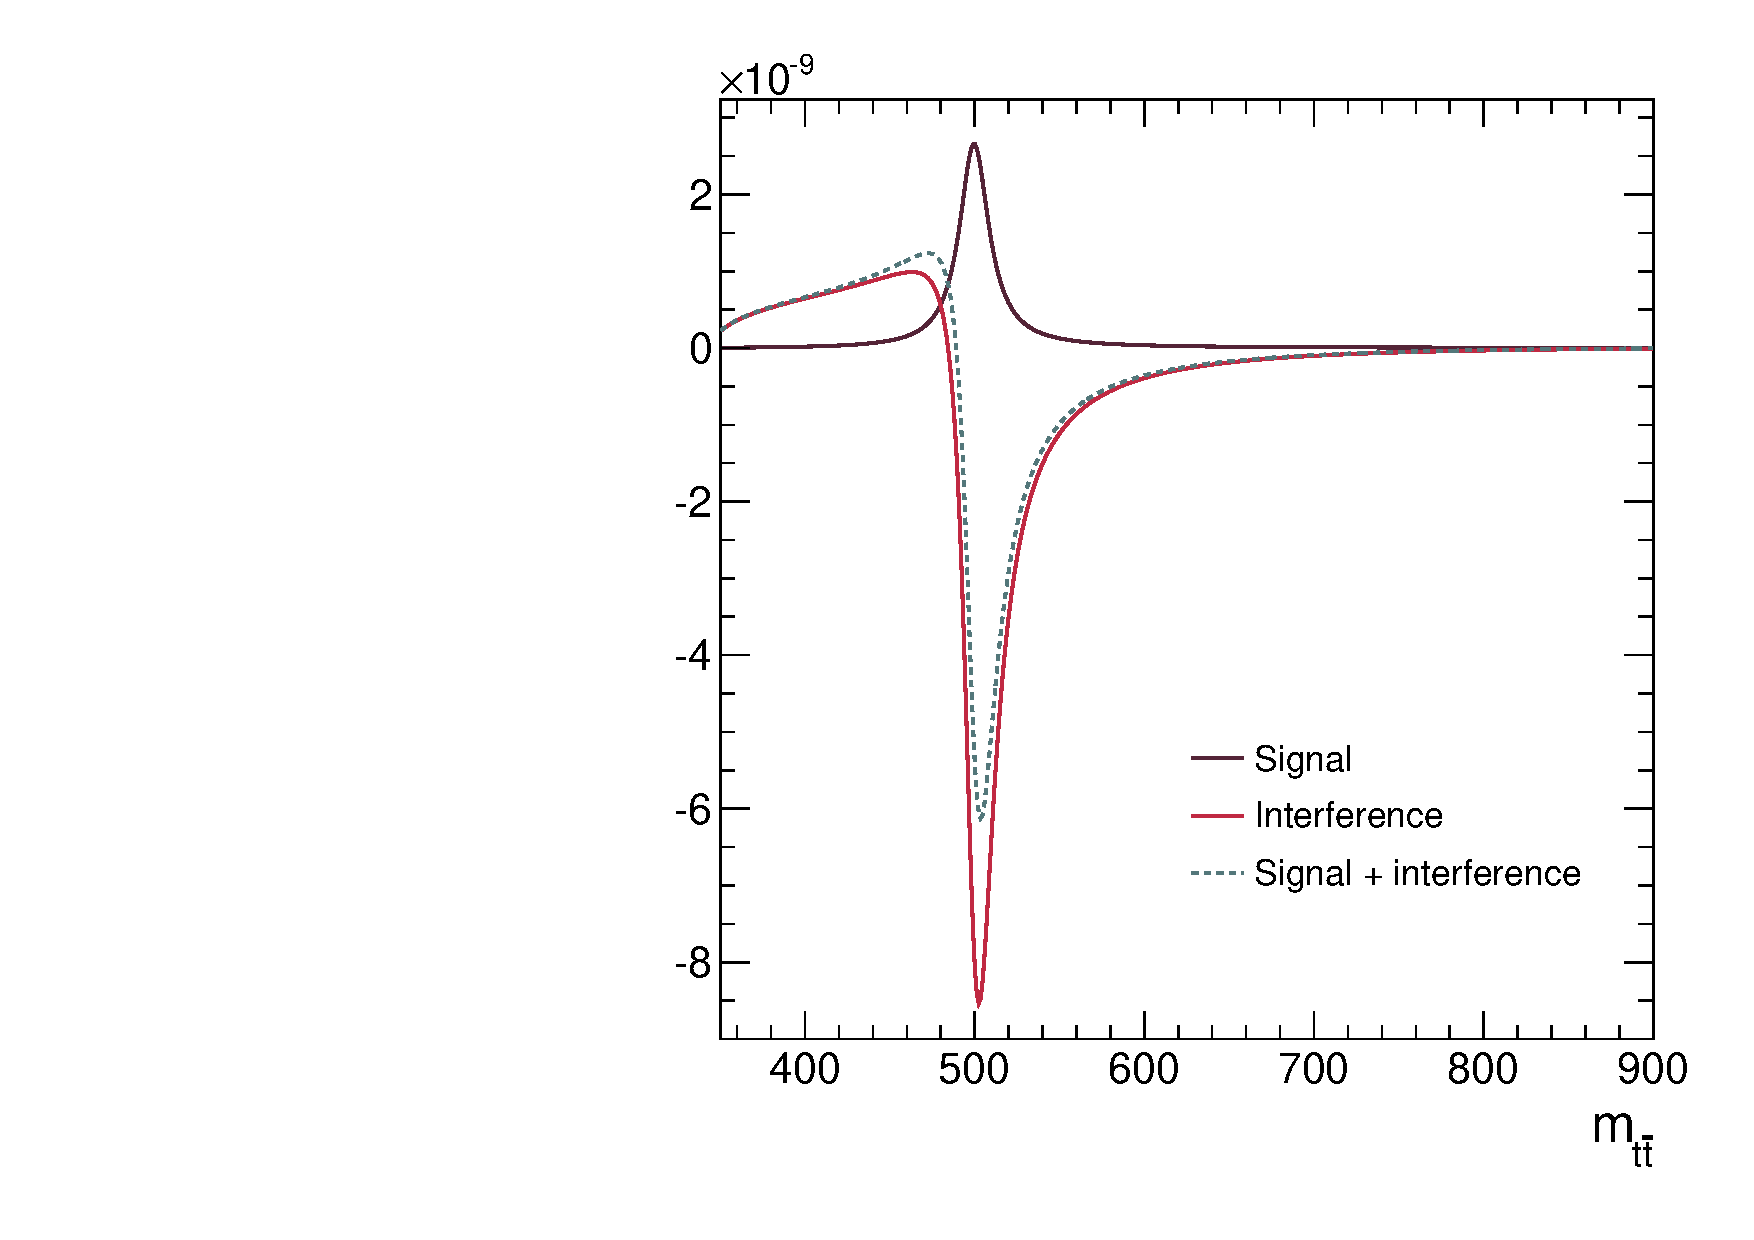
\includegraphics[width=0.48\textwidth,angle=-90,origin=c]{chapitre8/figs/S0/theory_pseudscalar_500_sig_int.pdf}}
    \caption{Section efficace pour le signal (courbe \verte), l'interférence (courbe \oranged), et pour signal + interférences (courbe pointillée \grise), obtenue à l'aide des \cref{eq:sigma_scalar,eq:sigma_pscalar}, pour la désintégration $\sz \rightarrow \ttbar$ en fonction de \mtt, pour $\msz = \SI{500}{\GeV}$. Les PDFs des partons ne sont pas incluses dans le calcul.}
    \label{fig:signal_interference}
\end{figure}

\smallskip

Afin de reproduire ce phénomène d'interférence, il est nécessaire, lors de la génération du signal, de le générer avec le bruit de \ttbar Modèle Standard. Le nombre d'événements générés nécessaires dans cette configuration n'est pas compatible avec les ressources disponibles. En effet, si l'on souhaite obtenir une luminosité équivalente pour le signal d'environ \SI{100}{\invfb}, il est nécessaire de générer environ \num{25000000} événements par points de masses. Pour que l'analyse soit possible, il est donc impératif de pouvoir générer uniquement les composantes dues au signal et aux interférences.

\bigskip

Lors de la génération du signal, quatre diagrammes interviennent dans le calcul de l'élément de matrice à l'arbre. Ces diagrammes sont présentés dans la \cref{fig:f_interference}. L'élément de matrice total est donné par
\begin{align*}
  \mathcal{M}^2 &\propto \abs{\mathcal{M}_a + \mathcal{M}_b + \mathcal{M}_c + \mathcal{M}_d}^2
\end{align*}

On modifie l'élément de matrice afin de ne garder que le signal et les termes interférant avec celui-ci. On obtient ainsi
%\setcounter{equation}{2}
\begin{align} \label{eq:matrix_element_higgs}
  \mathcal{M}^2 &\propto \mathcal{M}_a^2 + \mathcal{M}_a\mathcal{M}_b^\ast + \mathcal{M}_a\mathcal{M}_c^\ast + \mathcal{M}_a\mathcal{M}_d^\ast + \text{complexe conjugué}.
\end{align}

\begin{figure}[btp] \centering
    \subcaptionbox{\label{fig:f_signal} Signal}[0.48\textwidth]{\fmfreuse{higgs}}\hfill
    \subcaptionbox{\label{fig:f_bkg_1} Fond}[0.48\textwidth]{
    \begin{fmfgraph*}(160,70)
        \fmfstraight
        \fmfpen{0.5}
        \fmfleftn{i}{2} \fmfrightn{o}{2}
        \fmf{gluon}{i1,v1,i2}
        \fmf{gluon}{v1,v2}
        \fmf{fermion}{o1,v2,o2}
        \fmfv{label=\Ptop}{o1}
        \fmfv{label=\APtop}{o2}
        \fmfdotn{v}{2}
    \end{fmfgraph*}
    } \\ \vspace{5mm}
    \subcaptionbox{\label{fig:f_bkg_2} Fond}[0.48\textwidth]{
    \begin{fmfgraph*}(160,70)
        \fmfstraight
        \fmfpen{0.5}
        \fmfleftn{i}{2} \fmfrightn{o}{2}
        \fmf{gluon}{i1,v1}
        \fmf{fermion}{v1,o1}
        \fmf{gluon}{i2,v2}
        \fmf{fermion}{o2,v2}
        \fmf{fermion,label=\APtop}{v2,v1}
        \fmfv{label=\Ptop}{o1}
        \fmfv{label=\APtop}{o2}
        \fmfdotn{v}{2}
    \end{fmfgraph*}
    } \hfill
    \subcaptionbox{\label{fig:f_bkg_3} Fond}[0.48\textwidth]{
    \begin{fmfgraph*}(160,70)
        \fmfstraight
        \fmfpen{0.5}
        \fmfleftn{i}{2} \fmfrightn{o}{2}
        \fmf{gluon}{i1,v1}
        \fmf{fermion}{o1,v1}
        \fmf{gluon}{i2,v2}
        \fmf{fermion}{v2,o2}
        \fmf{fermion,label=\Ptop}{v1,v2}
        \fmfv{label=\Ptop}{o2}
        \fmfv{label=\APtop}{o1}
        \fmfdotn{v}{2}
    \end{fmfgraph*}
    }
    \caption{Diagrammes de Feynman des processus intervenants dans le calcul de l'élément de matrice pour la génération du signal.}
    \label{fig:f_interference}
\end{figure}

Le signal est généré à l'aide de \texttt{MadGraph\;5}. Le code généré et responsable du calcul de l'élément de matrice est modifié manuellement afin de correspondre à l'\cref{eq:matrix_element_higgs}.

Afin de valider cette méthode, qui consiste a modifier l’élément de matrice, on procède aussi à une génération complète, où le signal et le bruit de fond sont générés ensemble et à laquelle on soustrait le bruit de fond généré séparément. Les distributions de masse invariante \mtt obtenues dans chacun des cas sont présentées sur la \cref{fig:mtt_check} pour un \sz scalaire de masse $\msz = \SI{500}{\GeV}$. Les deux générations donnent des résultats comparables, ce qui permet de valider notre méthode de génération du signal. Il est également intéressant de constater que les erreurs statistiques sont réduites d'un facteur \tilde8, et ce en générant un nombre d'événements 100 fois inférieur.

\begin{figure}[t!]
    \centering
    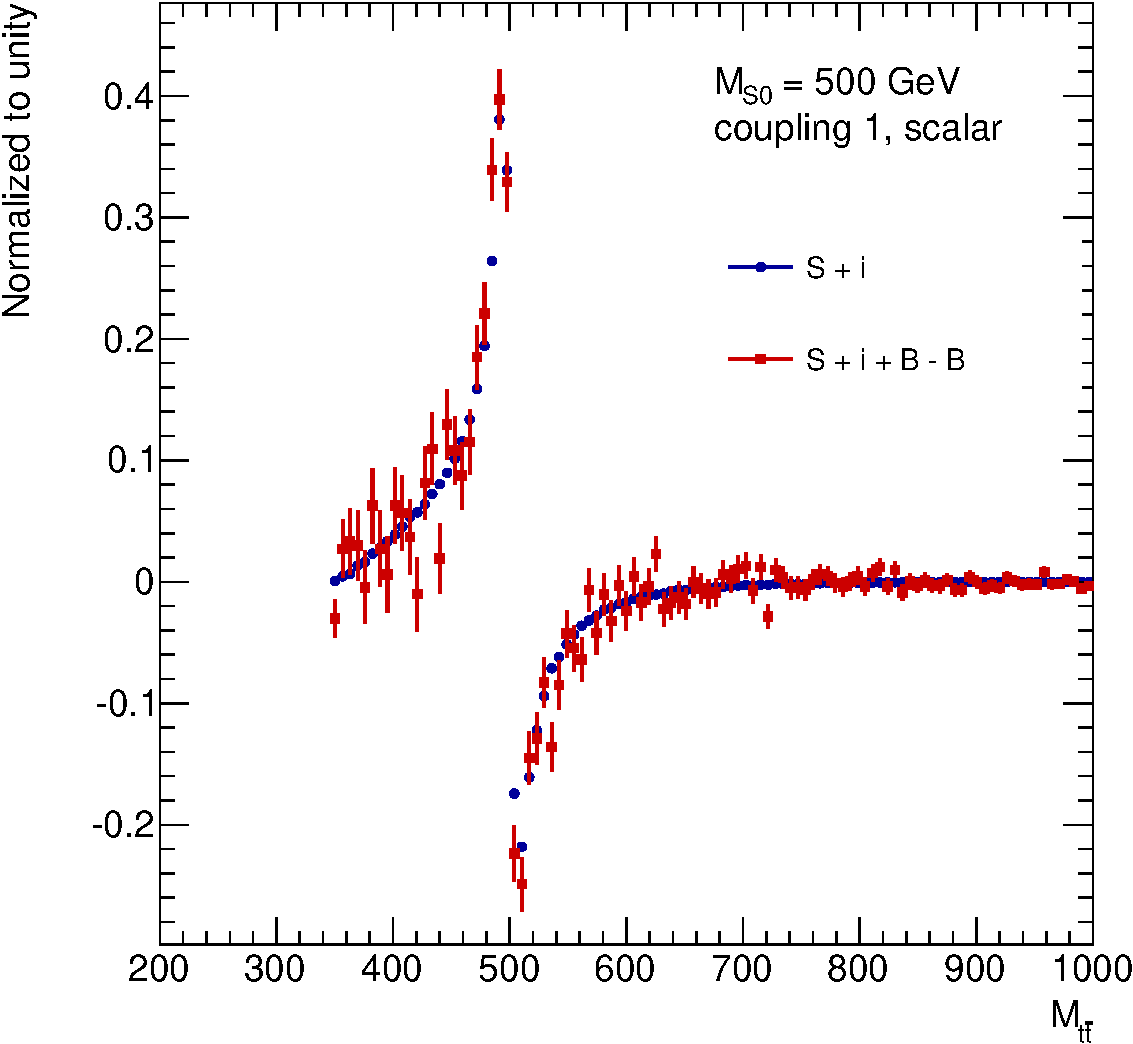
\includegraphics[width=0.6\textwidth]{chapitre8/figs/plot_overlaid_500_cpl1_S_i_B_plus_S_i_B_minus_B_more_stat.pdf}
    \caption{Distribution de masse invariante \mtt pour un \sz scalaire de masse $\msz = \SI{500}{\GeV}$, avec interférences. La distribution rouge est obtenue en générant le signal et le bruit de fond ensemble, puis en soustrayant le bruit de fond généré séparément. La distribution bleue est obtenue en générant uniquement le signal et les interférences, en modifiant le calcul de l'élément de matrice.}
    \label{fig:mtt_check}
\end{figure}

\begin{figure}[b!] \centering
    \subcaptionbox{Pseudo-scalaire, $\msz = \SI{400}{\GeV}$}[0.48\textwidth]{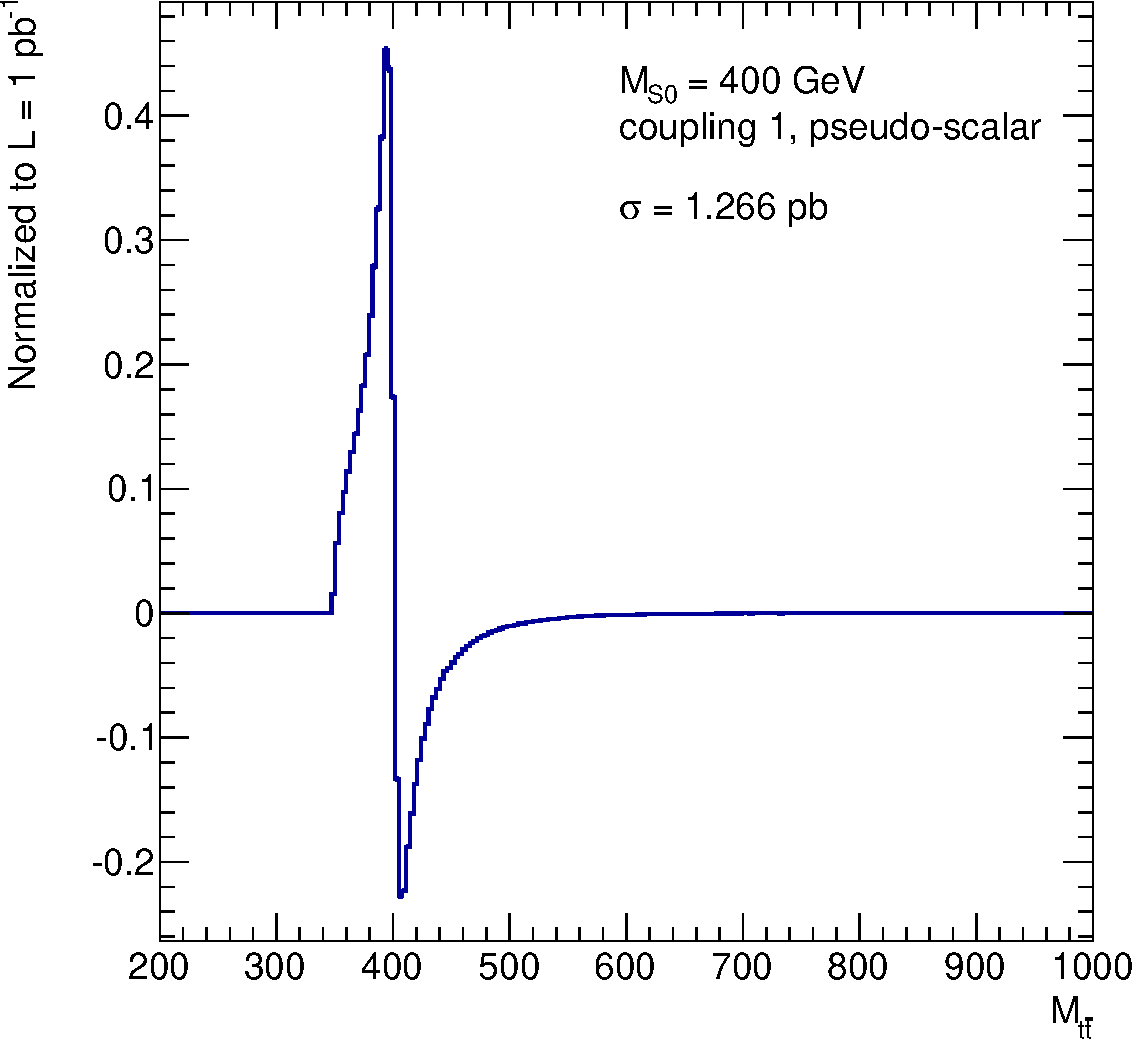
\includegraphics[width=0.48\textwidth]{chapitre8/figs/S0/plot_400_cpl1_pseudoscalar_normalized.pdf}} \hfill
    \subcaptionbox{Scalaire, $\msz = \SI{800}{\GeV}$}[0.48\textwidth]{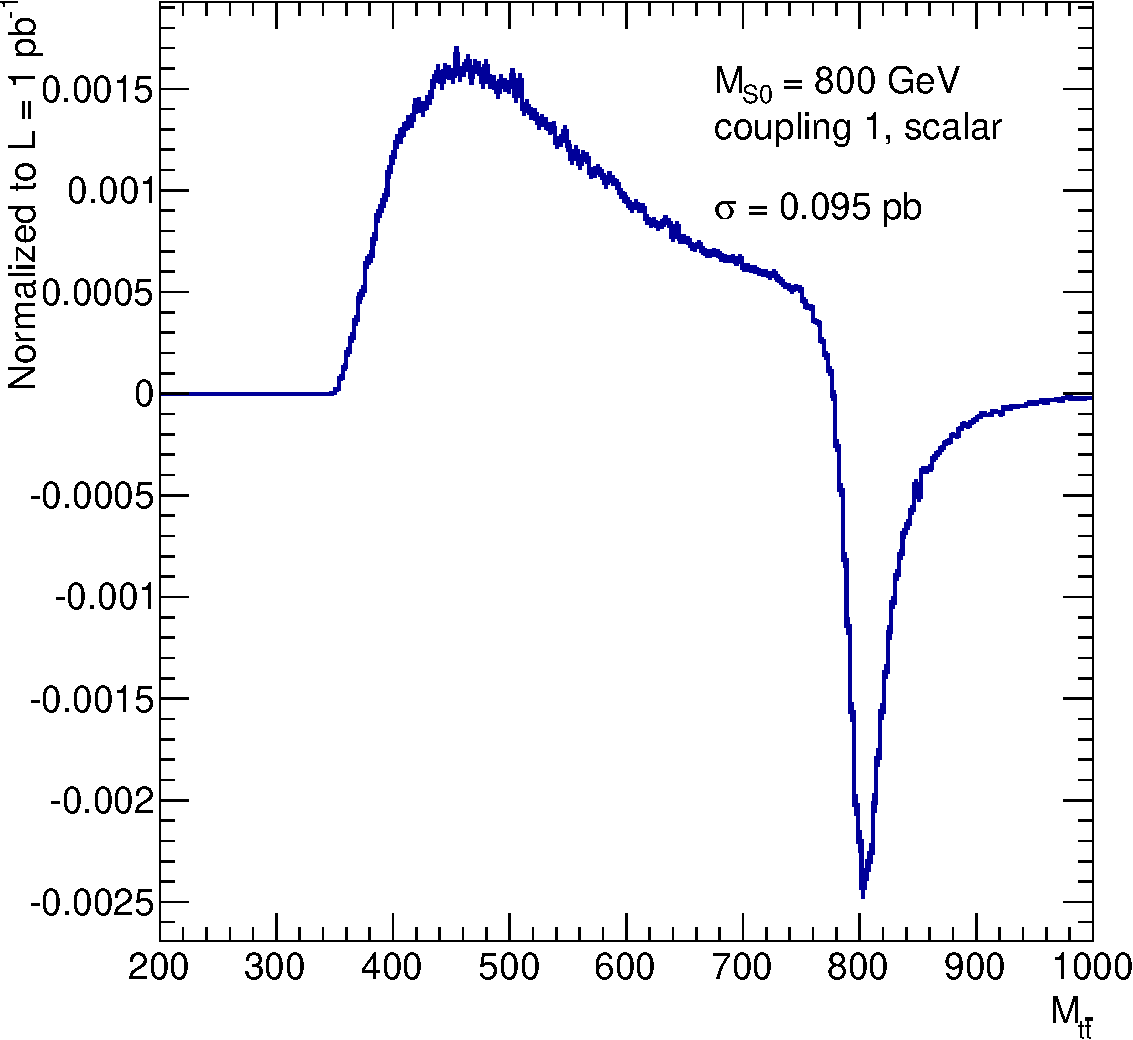
\includegraphics[width=0.48\textwidth]{chapitre8/figs/S0/plot_800_cpl1_normalized.pdf}}
    \caption{Distributions de masse invariante pour la désintégration $\sz \rightarrow \ttbar$, après la génération des événements par \texttt{MadGraph}.}
    \label{fig:gen_higgs}
\end{figure}

\bigskip

Chaque échantillon de signal utilisé dans cette analyse est généré à l'aide de la méthode alternative. On peut voir sur la \cref{fig:gen_higgs} les distributions de masse invariante pour un \sz scalaire et pseudo-scalaire après la génération. On note quelques différences avec les prédictions théoriques (\cref{fig:theo_sigma}), imputables aux densités de probabilités partoniques, utilisées lors de la génération des événements. Les sections efficaces de production à l'arbre prédites par \texttt{MadGraph} pour une production signal + interférences sont résumées dans le \cref{tab:cross_sections}. Ces sections efficaces doivent être interprétées comme $\sigma - \sigma_\text{\ttbar}$, et elles sont proportionnelles au nombre d'événements observés, intégrés sur le spectre \mtt. L'excès et le déficit contribuent donc avec un signe opposé aux sections efficaces. Cependant, dans l'étude de la distribution \mtt, la présence de l'un et de l'autre permet d'observer un éventuel signal. Il n'est donc pas aisé d'interpréter les valeurs dans le \cref{tab:cross_sections} en terme de sensibilité à la présence de nouvelle physique.


\begin{table}[t] \centering
    \begin{tabular}{cccccc} \toprule
     & \SI{400}{\GeV} & \SI{500}{\GeV} & \SI{600}{\GeV} & \SI{700}{\GeV} & \SI{800}{\GeV} \\ \midrule
     $\sigma_{\text{scalaire}}$ & \SI{0.5289}{\pb} & \SI{0.3023}{\pb} & \SI{0.1891}{\pb} & \SI{0.1295}{\pb} & \SI{0.0944}{\pb} \\
     $\sigma_{\text{pseudo-scalaire}}$ & \SI{1.169}{\pb} & \SI{0.6756}{\pb} & \SI{0.4414}{\pb} & \SI{0.3121}{\pb} & \SI{0.2325}{\pb} \\
     \bottomrule
    \end{tabular}
    \caption{Sections efficaces de production à l'arbre d'un Higgs scalaire ou pseudo-scalaire telles que prédites par \texttt{MadGraph}, pour un rapport d'embranchement en \ttbar de \SI{100}{\percent}, dans le cas d'une génération signal + interférences.}
    \label{tab:cross_sections}
\end{table}

\section{Sélection et reconstruction des événements}

La sélection des événements est identique à celle décrite dans le chapitre précédent, plus particulièrement dans la \cref{sec:zprime_sel}. Seule la coupure sur l'impulsion transverse des jets est différente.

Cette coupure dépend maintenant de la période de prise de données, à cause de changements dans la définition des chemins de déclenchement. On demande toujours au moins 4 jets, et
\begin{itemize}
    \item Pour les \emph{runs} A et B : $\pt > 45\,/\,45\,/\,45\,/\,\SI{30}{\GeV}$
    \item Pour les \emph{runs} C et D : $\pt > 55\,/\,45\,/\,35\,/\,\SI{30}{\GeV}$
\end{itemize}
Les coupures sur les deux premiers jets étant plus lâches, la reconstruction du signal à basse masse (\SI{400}{\GeV}) est plus efficace.

\smallskip

Les événements passant la sélection sont ensuite classés en 4 catégories, selon la saveur du lepton et le nombre de jets étiquetés \Pbottom :
\begin{center}
  \begin{tabular}{c} \toprule
    muon \\
    électron \\ \bottomrule
  \end{tabular} \qquad $\otimes$ \qquad
  \begin{tabular}{c} \toprule
    Exactement 1 jet étiqueté \Pbottom \\
    Au moins 2 jets étiquetés \Pbottom \\ \bottomrule
  \end{tabular}
\end{center}

Les techniques utilisées pour reconstruire l'événement \ttbar sont détaillées dans le \cref{chap:mtt_reco}.

Au moment de la génération du signal, un poids est associé à chaque événement. Ce poids peut être positif ou négatif selon si l'événement est un excès ou un déficit par rapport à la prédiction du Modèle Standard. Le fait qu'un événement puisse posséder un poids négatif affecte directement l'efficacité de sélection. Ce problème sera discuté en détails dans la \cref{sec:higgs_sel_eff}.

\begin{figure}[tbp] \centering
    \subcaptionbox{Scalaire}[0.48\textwidth]{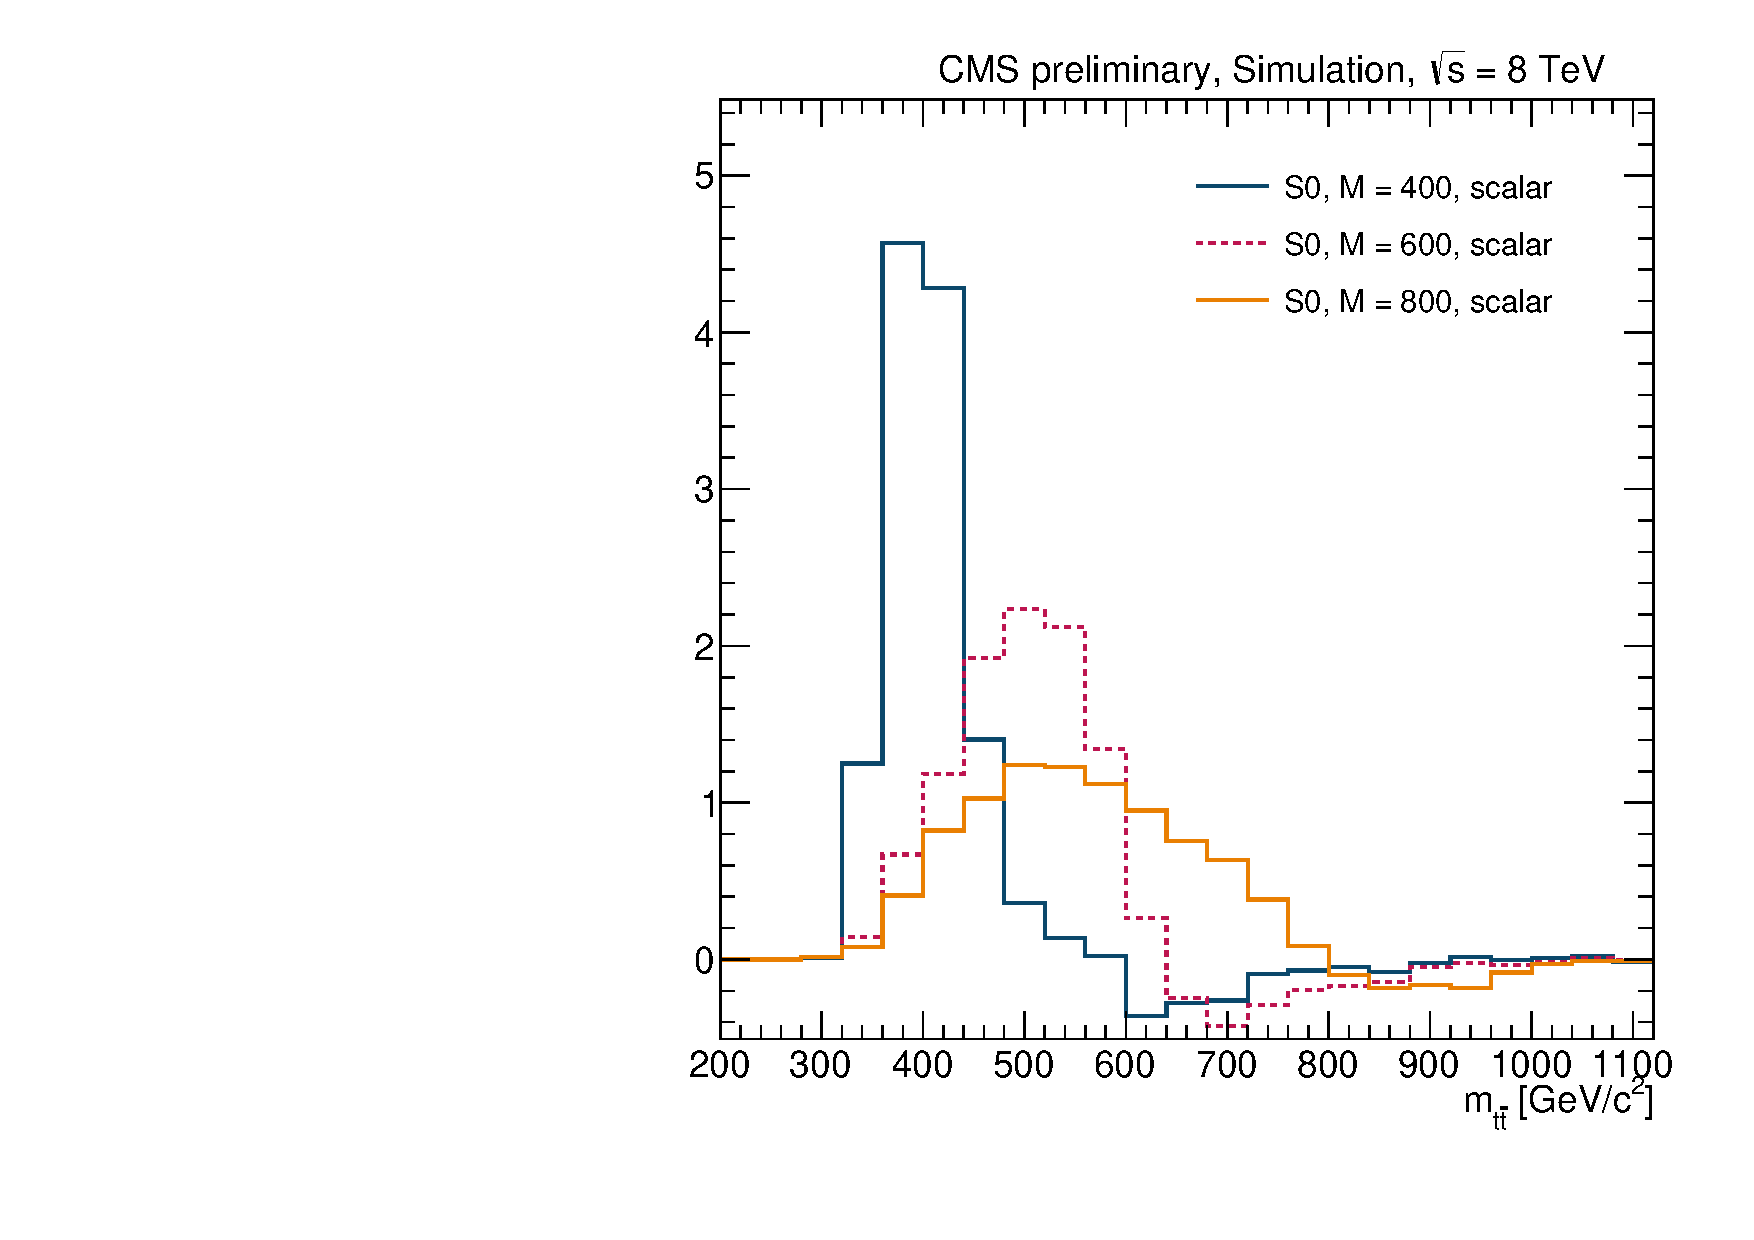
\includegraphics[width=0.48\textwidth,origin=c,angle=-90]{chapitre8/figs/scalar/mttSelected_btag_sel_reco_fullsel.pdf}} \hfill
    \subcaptionbox{Pseudo-scalaire}[0.48\textwidth]{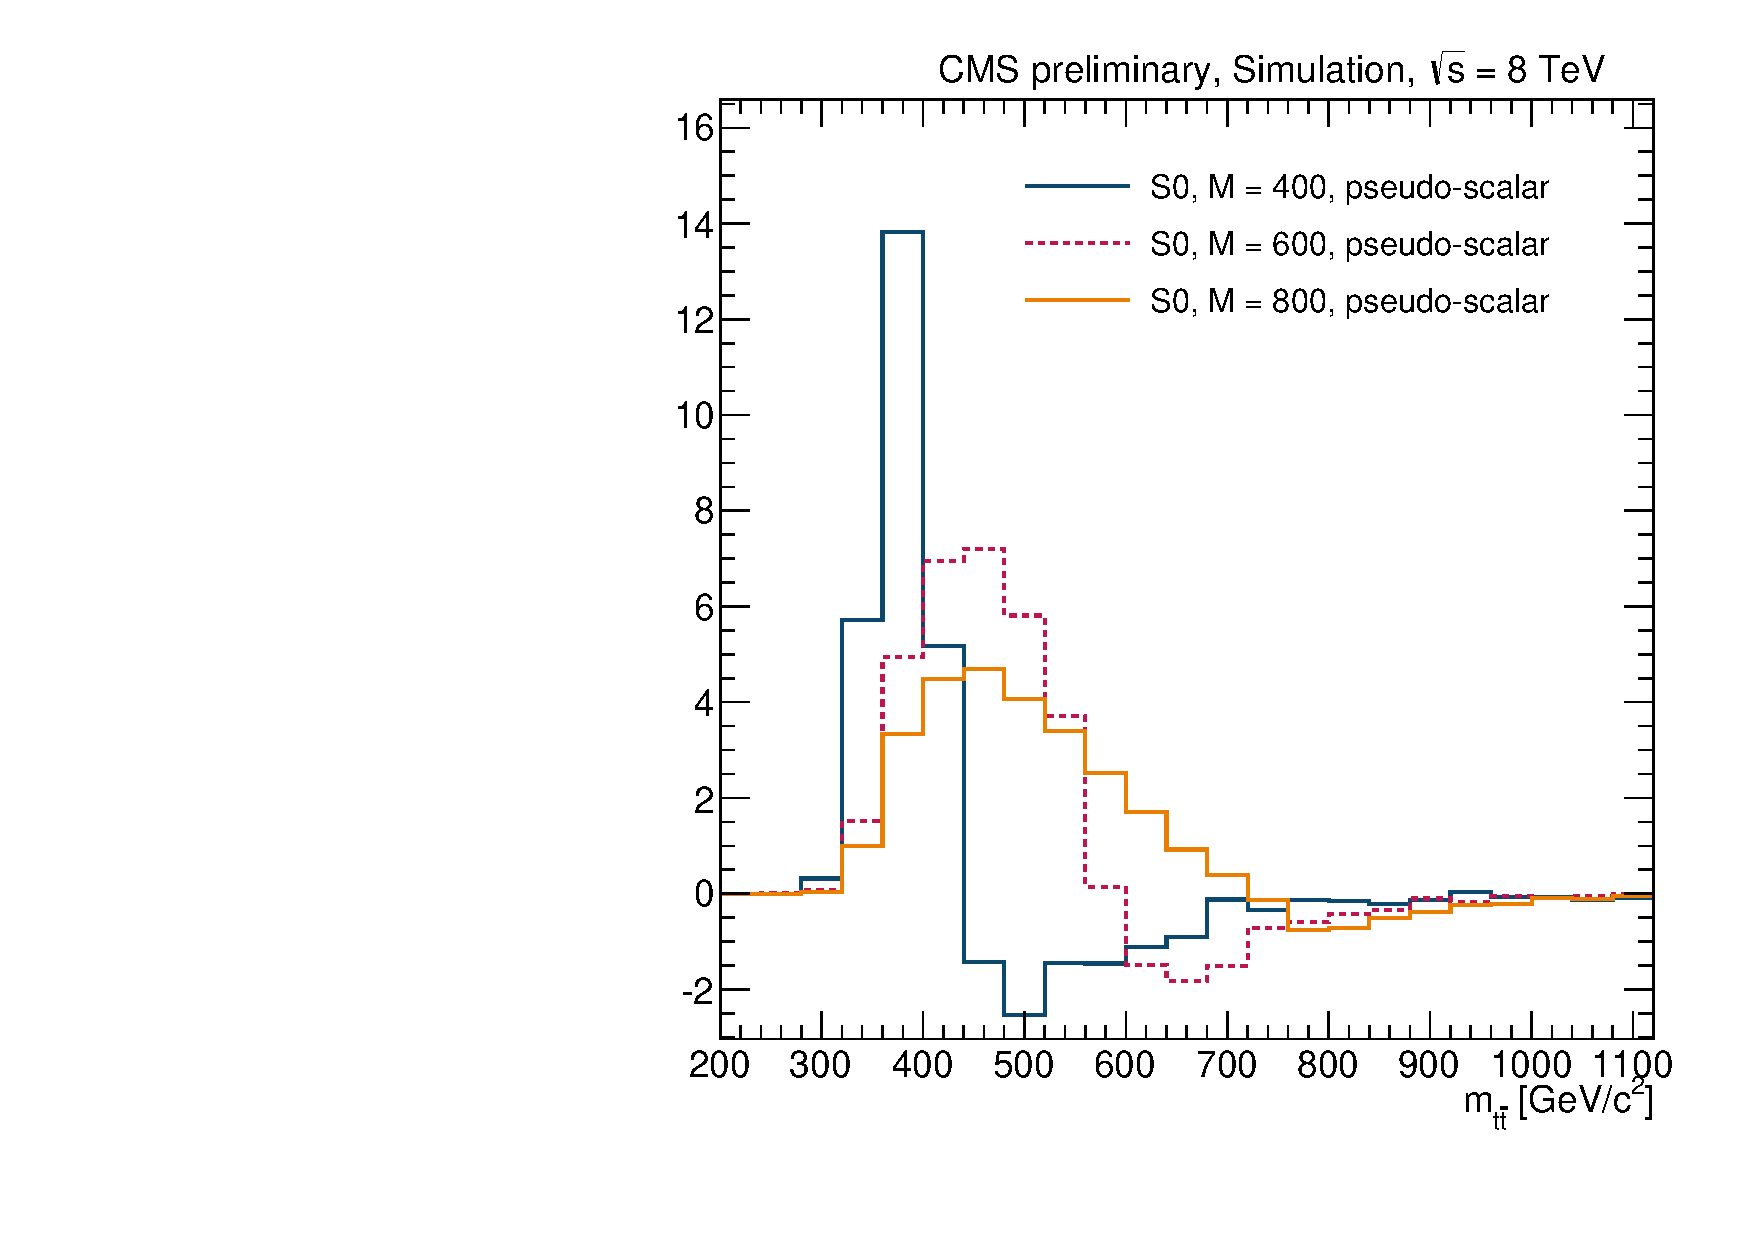
\includegraphics[width=0.48\textwidth,origin=c,angle=-90]{chapitre8/figs/pseudoscalar/mttSelected_btag_sel_reco_fullsel.pdf}}
    \caption{Distribution de masse invariante \mtt pour un \sz de masse $\msz = \SI{400}{\GeV}$ (\bleu), $\msz = \SI{600}{\GeV}$ (\rouge) et $\msz = \SI{800}{\GeV}$ (\orange), après sélection et reconstruction.}
    \label{fig:higgs_sig_reco}
\end{figure}

La distribution de masse invariante \mtt du signal après sélection et reconstruction est visible sur la \cref{fig:higgs_sig_reco}, pour différentes masses de signal. On constate que l'excès est clairement visible après reconstruction, et le déficit atténué.% On verra dans la \cref{sec:higgs_sel_eff} que, même si la partie négative de l'interférence n'est plus significative après reconstruction, l'effet de la présence d'interférences n'est pas sans effet pour notre analyse.

\section{Performance de la sélection}

\subsection{Efficacité des chemins de déclenchement}

A cause du changement de coupure sur l'impulsion transverse, il est possible d'utiliser les efficacités des chemins de déclenchement de référence de la collaboration, calculées directement sur les données. Pour le canal semi-muonique, l'efficacité moyenne obtenue est de \SI{89,5}{\percent}, et de \SI{94,3}{\percent} pour le canal semi-électronique. Si l'on compare ces valeurs aux efficacités obtenues dans l'analyse \zprime (voir \cref{sec:zp_eff_hlt}), on remarque qu'elles sont légèrement plus faibles, à cause des coupures sur l'impulsion transverse des jets plus lâches.

\subsection{Efficacité de la sélection} \label{sec:higgs_sel_eff}

La présence de poids négatifs nous oblige à modifier la façon dont on calcule l'efficacité de sélection. Si on définit l'efficacité de sélection comme le rapport entre le nombre d'événements sélectionnés (équivalent à l'intégrale de la distribution de masse invariante) et le nombre d'événements générés, on obtient sur le signal et ses interférences
\begin{align*}
  \epsilon &= \frac{N_A - N_B}{N_\text{généré}}
\end{align*}
où $N_A$ est le nombre d'événements positifs et $N_B$ le nombre d'événements négatifs (voir \cref{fig:int_eff}). Or, on souhaite quantifier une déviation par rapport à la prédiction du Modèle Standard : un événement négatif contribue tout autant à la déviation qu'un événement positif. On définit donc l'efficacité de sélection par
\begin{align*}
  \epsilon &= \frac{N_A + N_B}{N_\text{généré}}.
\end{align*}
\begin{figure}[tbp]
    \centering
    \includegraphics[width=0.6\textwidth]{chapitre8/figs/interferences.pdf}
    \caption{Exemple d'interférence produit par un processus de nouvelle physique sur un prédiction Modèle Standard. La zone A correspond à un excès d'événement, et la zone B à un déficit d'événement par rapport au Modèle Standard.}
    \label{fig:int_eff}
\end{figure}

\begin{table}[p] \centering
  \begin{tabular}{ccccccc} \toprule
    & \SI{400}{\GeV} & \SI{500}{\GeV} & \SI{600}{\GeV} & \SI{700}{\GeV} & \SI{800}{\GeV} \\ \midrule
    \multicolumn{3}{l}{Exactement 1 jet étiqueté \Pbottom} \\ \cmidrule{1-3}
    $\epsilon$, semi-$\mu$ & \num{0.168 \pm 0.003} & \num{0.230 \pm 0.003} & \num{0.357 \pm 0.004} & \num{0.464 \pm 0.005} & \num{0.589 \pm 0.005}\\
    $\epsilon$, semi-e & \num{0.141 \pm 0.003} & \num{0.193 \pm 0.003} & \num{0.294 \pm 0.004} & \num{0.400 \pm 0.004} & \num{0.504 \pm 0.005} \\ \midrule
    \multicolumn{3}{l}{Au moins 2 jets étiquetés \Pbottom} \\ \cmidrule{1-3}
    $\epsilon$, semi-$\mu$ & \num{0.138 \pm 0.003} &  \num{0.200 \pm 0.003} &  \num{0.313 \pm 0.004} & \num{0.416 \pm 0.005} & \num{0.519 \pm 0.005} \\
    $\epsilon$, semi-e & \num{0.119 \pm 0.002} &  \num{0.171 \pm 0.003} & \num{0.264 \pm 0.003} & \num{0.354 \pm 0.004} & \num{0.448 \pm 0.005} \\
    \bottomrule
  \end{tabular}
  \caption{Efficacités de sélection (en pourcent) du signal pour différentes masses de \sz scalaire. Ces efficacités sont calculés par rapport à la désintégration $\sz \rightarrow \ttbar$ inclusive.}
  \label{tab:eff_scalar}
\end{table}

\begin{table}[p] \centering
  \begin{tabular}{ccccccc} \toprule
    & \SI{400}{\GeV} & \SI{500}{\GeV} & \SI{600}{\GeV} & \SI{700}{\GeV} & \SI{800}{\GeV} \\ \midrule
    \multicolumn{3}{l}{Exactement 1 jet étiqueté \Pbottom} \\ \cmidrule{1-3}
    $\epsilon$, semi-$\mu$ & \num{0.176 \pm 0.003} & \num{0.341 \pm 0.004} & \num{0.504 \pm 0.005} & \num{0.668 \pm 0.006} & \num{0.772 \pm 0.006}\\
    $\epsilon$, semi-e & \num{0.148 \pm 0.003} & \num{0.288 \pm 0.004} & \num{0.436 \pm 0.005} & \num{0.576 \pm 0.005} & \num{0.656 \pm 0.006} \\ \midrule
    \multicolumn{3}{l}{Au moins 2 jets étiquetés \Pbottom} \\ \cmidrule{1-3}
    $\epsilon$, semi-$\mu$ & \num{0.156 \pm 0.003} & \num{0.301 \pm 0.004} & \num{0.446 \pm 0.005} & \num{0.583 \pm 0.005} & \num{0.657 \pm 0.006}\\
    $\epsilon$, semi-e & \num{0.130 \pm 0.002} & \num{0.252 \pm 0.004} & \num{0.374 \pm 0.004} & \num{0.480 \pm 0.005} & \num{0.558 \pm 0.005}\\
    \bottomrule
  \end{tabular}
  \caption{Efficacités de sélection (en pourcent) du signal pour différentes masses de \sz pseudo-scalaire. Ces efficacités sont calculés par rapport à la désintégration $\sz \rightarrow \ttbar$ inclusive.}
  \label{tab:eff_pseudoscalar}
\end{table}

Les efficacités de sélection sont résumées dans les \cref{tab:eff_scalar,tab:eff_pseudoscalar}. On constate que ces efficacités sont plus faibles que celles obtenues dans l'analyse \zprime (voir \cref{sec:zprime_eff_sel}), à cause de la présence d'interférences. En effet, un événement auquel le générateur assigne un poids négatif devrait contribuer au déficit. Après reconstruction, deux phénomènes peuvent se produire :
\begin{itemize}
    \item L'événement est reconstruit avec une masse invariante correcte, et contribue au déficit.
    \item L'événement est reconstruit avec une masse invariante différente de la masse invariante générée. Dans ce cas, il est possible d'obtenir l'effet inverse : au lieu de contribuer au déficit, l'événement va venir atténuer l'excès. L'inverse est également possible : un événement censé contribuer à l'excès peut venir atténuer le déficit à cause d'une mauvaise reconstruction.
\end{itemize}

\begin{figure}[tbp] \centering
    \subcaptionbox{Pseudo-scalaire, $\msz = \SI{400}{\GeV}$}[0.48\textwidth]{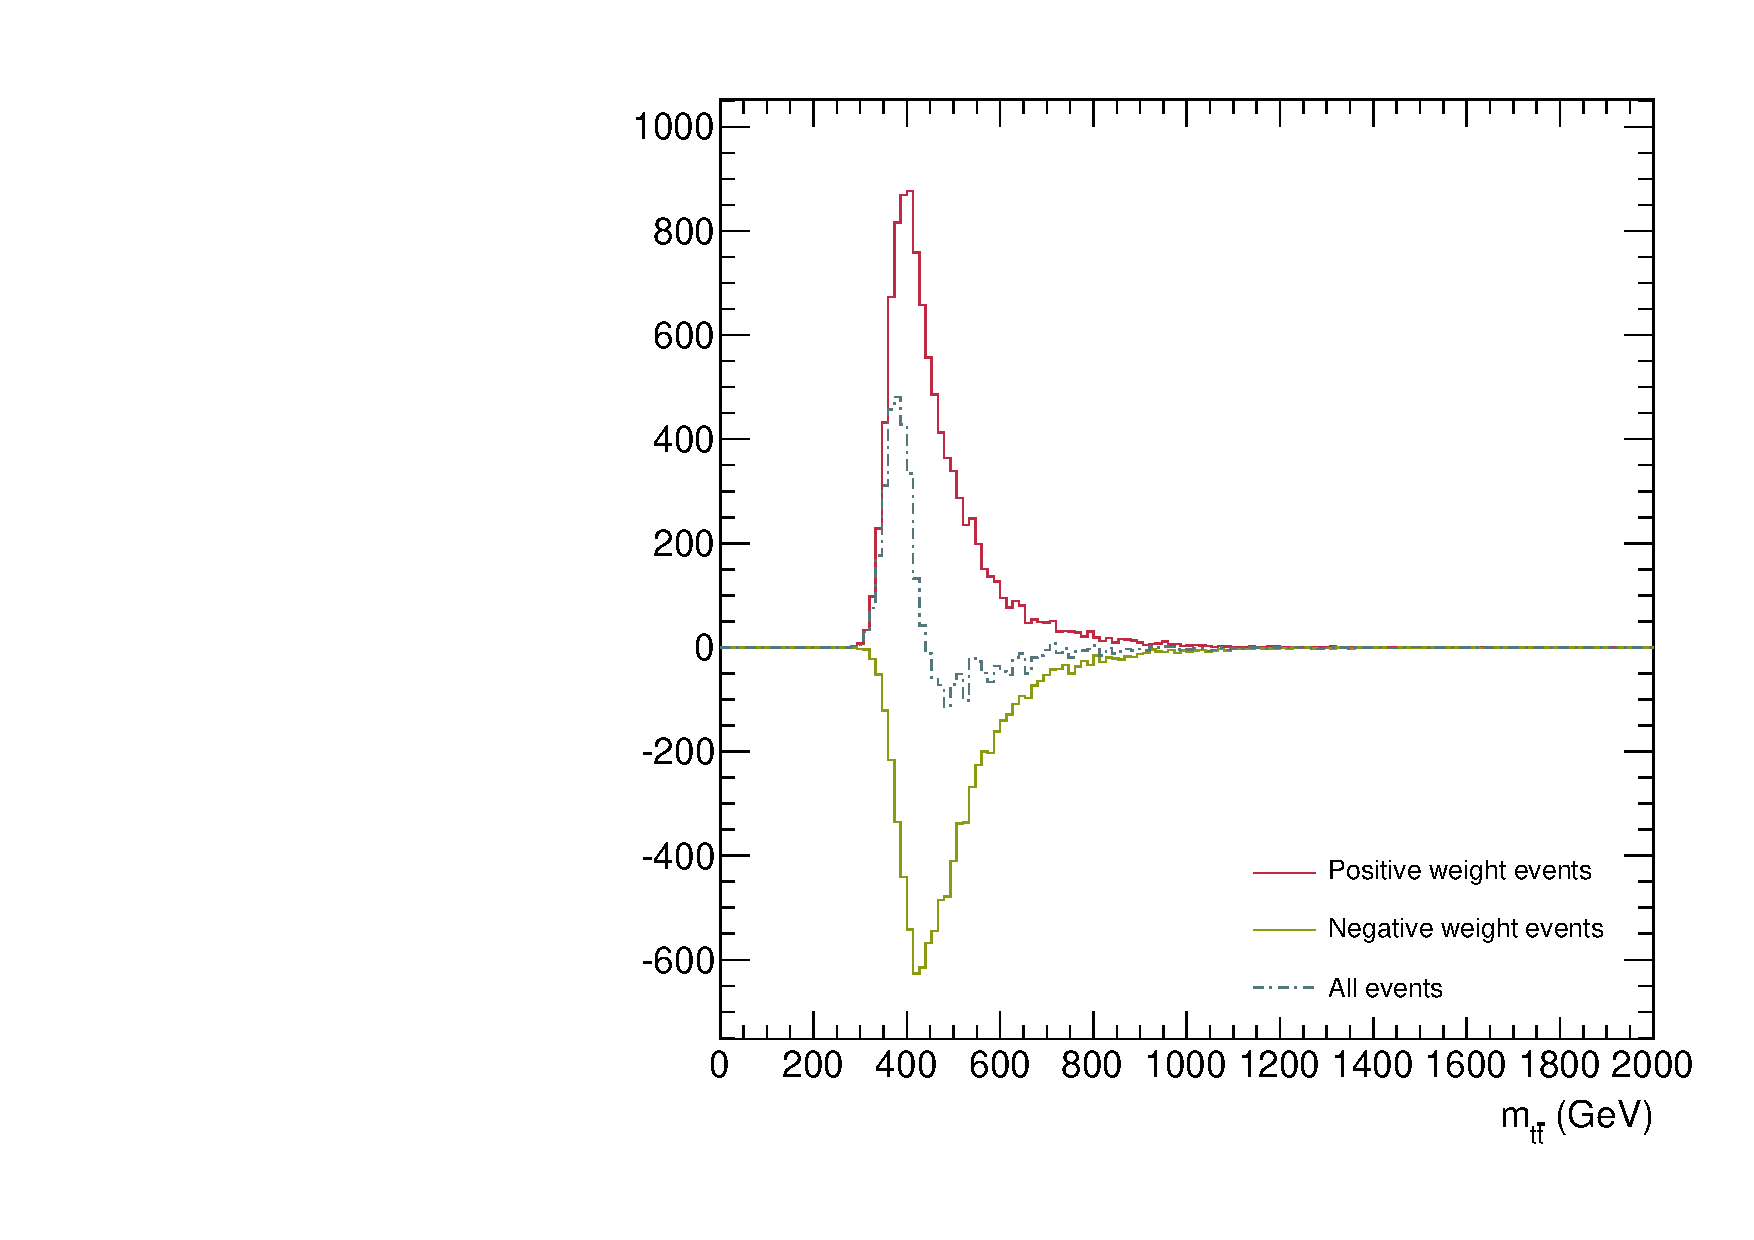
\includegraphics[width=0.48\textwidth,origin=c,angle=-90]{chapitre8/figs/S0/s0_positive_negative_pseudoscalar_400.pdf}}
    \subcaptionbox{Pseudo-scalaire, $\msz = \SI{800}{\GeV}$}[0.48\textwidth]{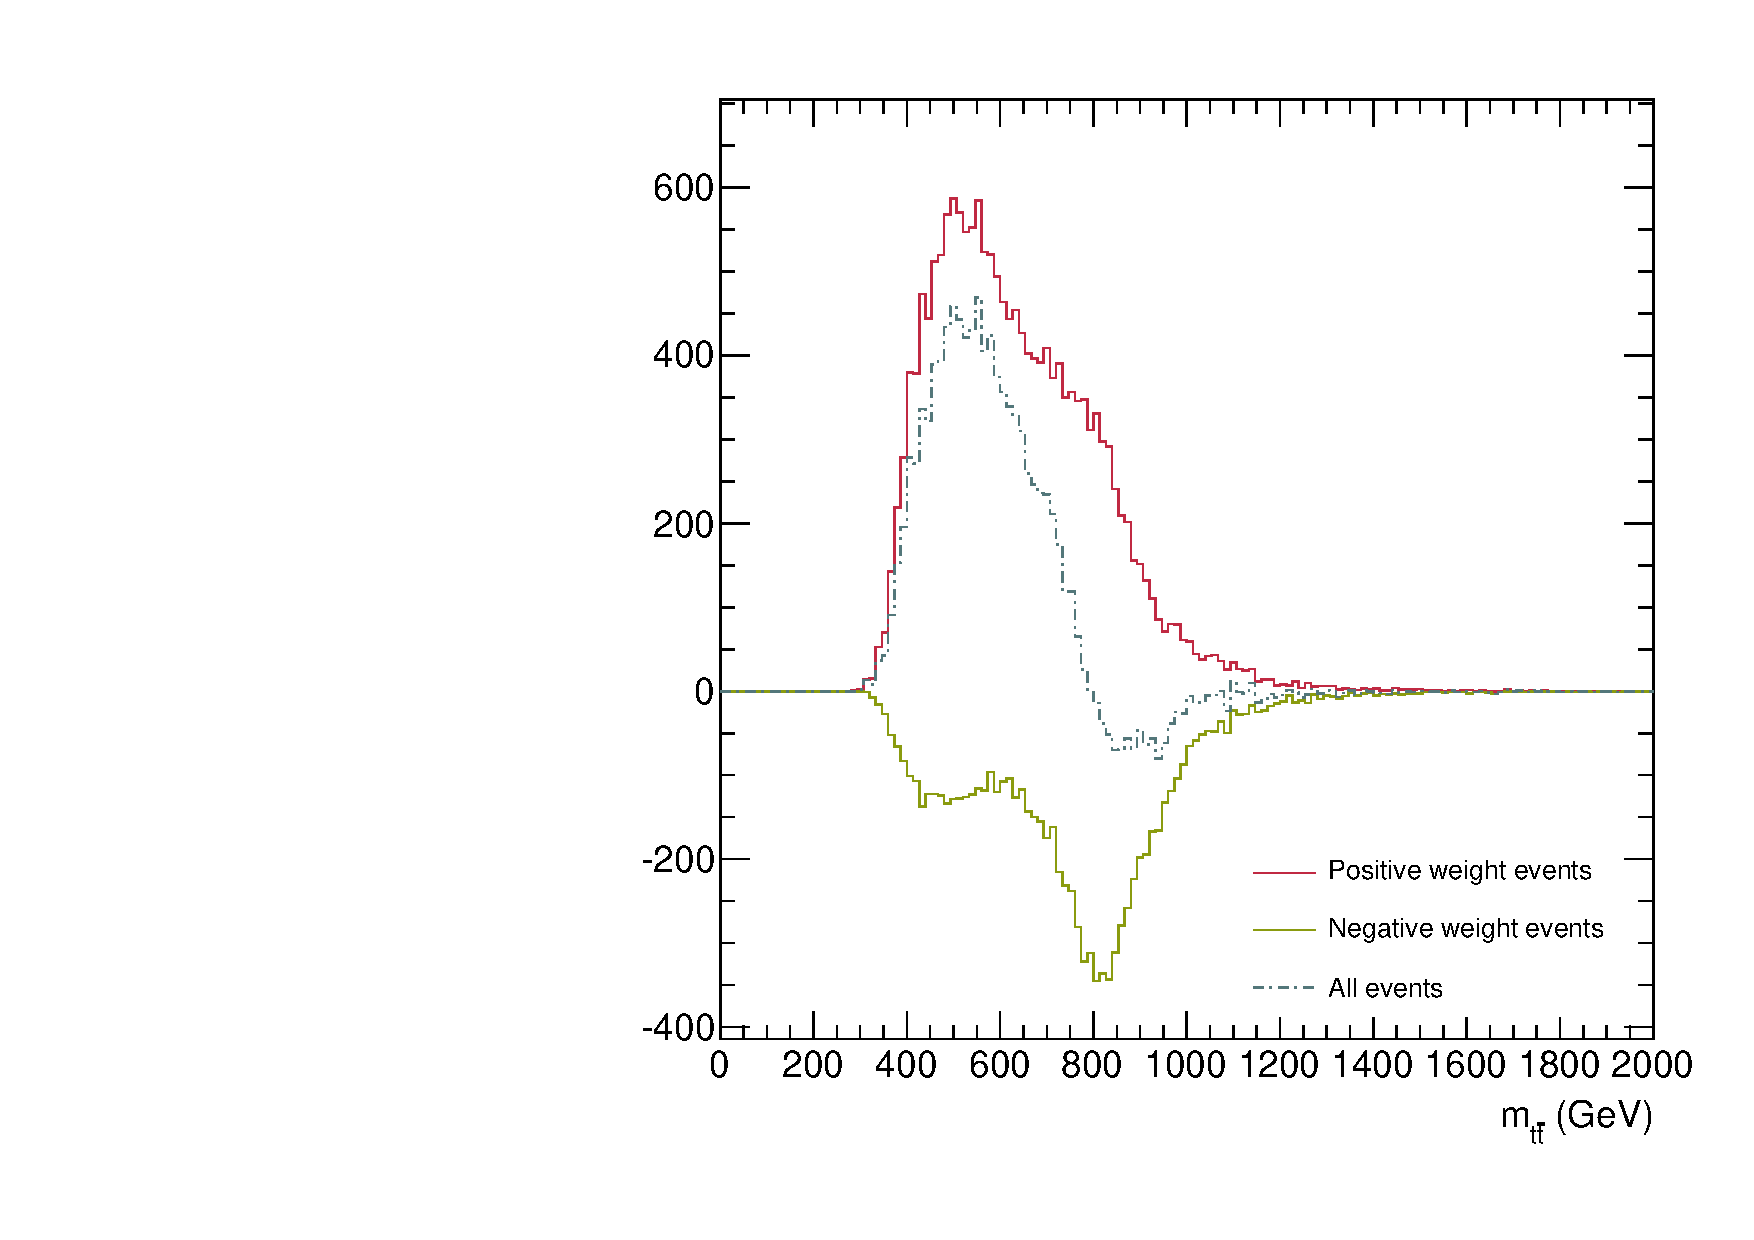
\includegraphics[width=0.48\textwidth,origin=c,angle=-90]{chapitre8/figs/S0/s0_positive_negative_scalar_800.pdf}}
    \caption{Effet des interférences sur la reconstruction du signal. Les événements avec un poids positif sont représentés en \rouge et ceux avec un poids négatif en \vertc. Le signal reconstruit, représenté en \gris, est obtenu en sommant les distributions \rouge et \vertc.}
    \label{fig:interference_effet}
\end{figure}

Cet effet est illustré sur la \cref{fig:interference_effet}. Si l'on compare avec les distributions obtenues au niveau générateur (\cref{fig:gen_higgs}), on constate très clairement que l'excès et le déficit sont élargies par la reconstruction. Le signal reconstruit, qui est simplement la somme de l'excès et du déficit, se trouve ainsi artificiellement atténué. Cette atténuation est d'autant plus importante que le recouvrement entre l'excès et le déficit est important. Ainsi, l'effet est maximal à \SI{400}{\GeV}, et diminue à mesure que la masse augmente, ce qui explique l'augmentation de l'efficacité de sélection avec la masse de la résonance.

Ainsi, la résolution sur la reconstruction de \mtt influe directement sur l'efficacité de sélection.

\bigskip

%On a pu voir que les interférences n'ont pas autant d'effet sur la forme du signal après reconstruction qu'au niveau générateur, la partie négative de l'interférence ayant disparu. Pour autant, il n'est pas possible de négliger ces interférences, au risque de surestimer considérablement les efficacités de sélection, et ainsi le pouvoir d'exclusion de l'analyse.

De manière analogue à l'analyse \zprime, des facteurs de corrections sont appliqués afin de prendre en compte les différences de performances de reconstruction entre les données et la simulation, telles que l'identification des leptons, l'algorithme d'étiquetage des jets de \Pbottom, ... Ces facteurs sont appliqués événement par événement, pour chaque bruit de fond et signal considérés : en plus de modifier la normalisation, ce changement permet de prendre en compte les possibles modifications de la forme des distributions.
% En moyenne:
% \begin{itemize}
%   \item Identification et isolation des muons : \num{0.992 \pm 0.005}.
%   \item Identification et isolation des électrons : \num{0.982 \pm 0.003}.
%   \item Étiquetage des jets de \Pbottom : \num{1.043 \pm 0.022} pour exactement 1 jet étiqueté \Pbottom, et \num{0.927 \pm 0.038} pour au moins deux jets étiquetés \Pbottom.
% \end{itemize}

\section{Stratégie de l'analyse}

La production de résonances de spin 0 se désintégrant en \ttbar intervient dès que $\msz = 2 m_{\Ptop} \simeq \SI{350}{\GeV}$. On étend ainsi notre gamme de masse invariante, et on considère dans cette analyse $\mtt \in \left[\SI{250}{\GeV}, \SI{1250}{\GeV}\right]$. Le nombre de classes en \mtt est choisi de façon à ce que la largeur de chaque classe soit de \SI{10}{\GeV}.

En analogie avec l'analyse \zprime, plusieurs fonctions analytiques ont été testées pour décrire le spectre de masse invariante de la production du Modèle Standard. En raison de l'absence de la coupure à \SI{550}{\GeV}, et donc d'une gamme en masse invariante qui n'est plus limitée à la partie uniquement décroissante, aucune fonction n'a été en mesure de produire un ajustement correct et non biaisé.

Au lieu d'estimer le bruit de fond directement sur les données, la simulation est utilisée pour décrire le spectre de masse invariante \mtt du Modèle Standard. Il est ainsi aisé de décrire toute la gamme de masse, puisque aucune fonction analytique n'est nécessaire. En contre\-/partie, cette méthode introduit plusieurs incertitudes systématiques qui n'étaient pas présentes dans l'analyse \zprime. Ces nouvelles incertitudes sont décrites dans la \cref{sec:higgs_syst}.

\section{Comparaisons données / simulation}

Les comparaisons entre les données et la simulation sont visibles sur la \cref{fig:higgs_data_mc}, pour \mtt et pour chacune des catégories de l'analyse. La simulation est normalisée aux valeurs de sorties d'un ajustement sur les données par la méthode du maximum de vraisemblance, présenté dans la \cref{sec:higgs_stat}. La zone hachurée grise correspond aux incertitudes statistiques et systématiques. Les comparaisons pour d'autres variables sont disponibles dans l'\cref{an:higgs_data_mc}. La valeur de chaque facteur de correction est résumé dans le \cref{tab:higgs_corr}.

% \begin{figure}[p!] \centering
%     \subcaptionbox{Canal semi-muonique}[0.49\textwidth]{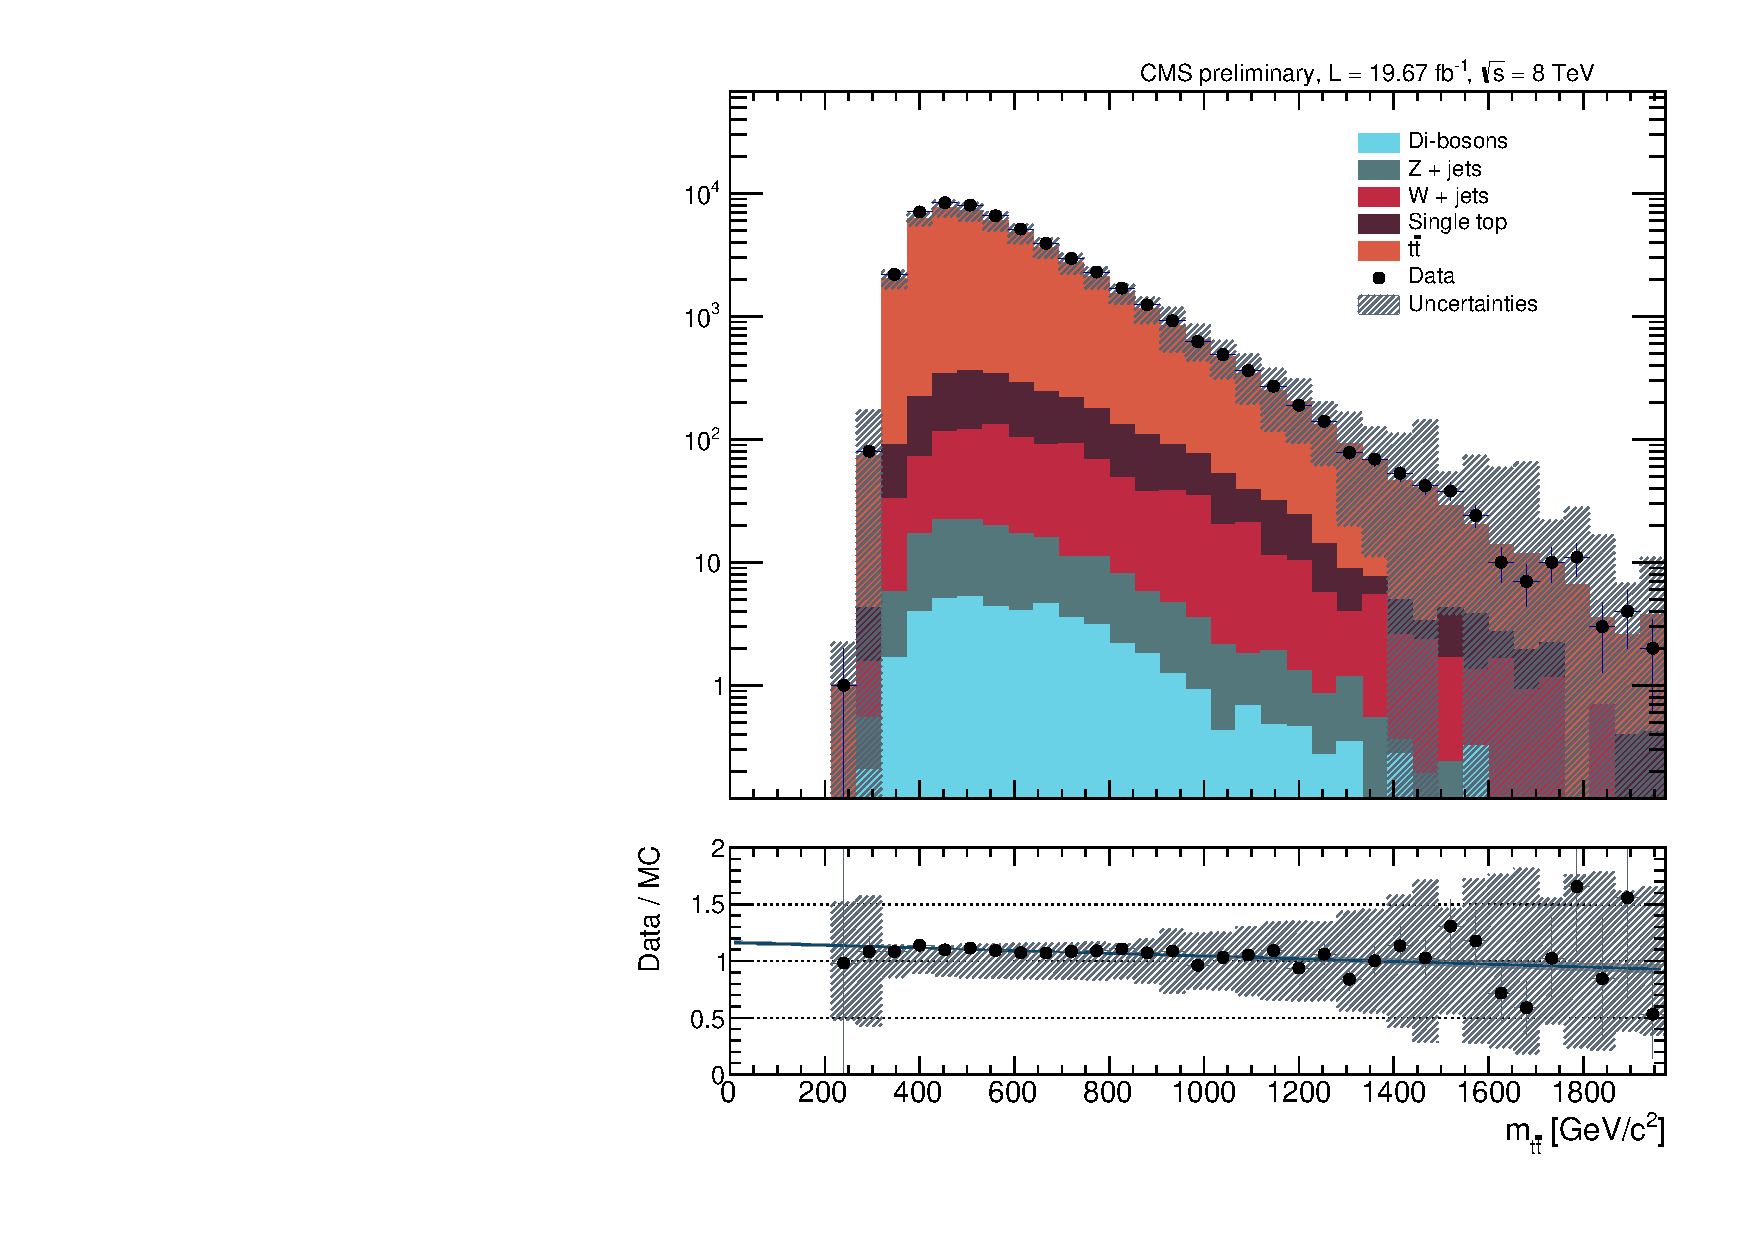
\includegraphics[width=0.49\textwidth,angle=-90,origin=c]{chapitre8/figs/data_mc_old_syst/2-btag/semimu/mttSelected_btag_sel_reco_fullsel.pdf}} \hfill
%     \subcaptionbox{Canal semi-électronique}[0.49\textwidth]{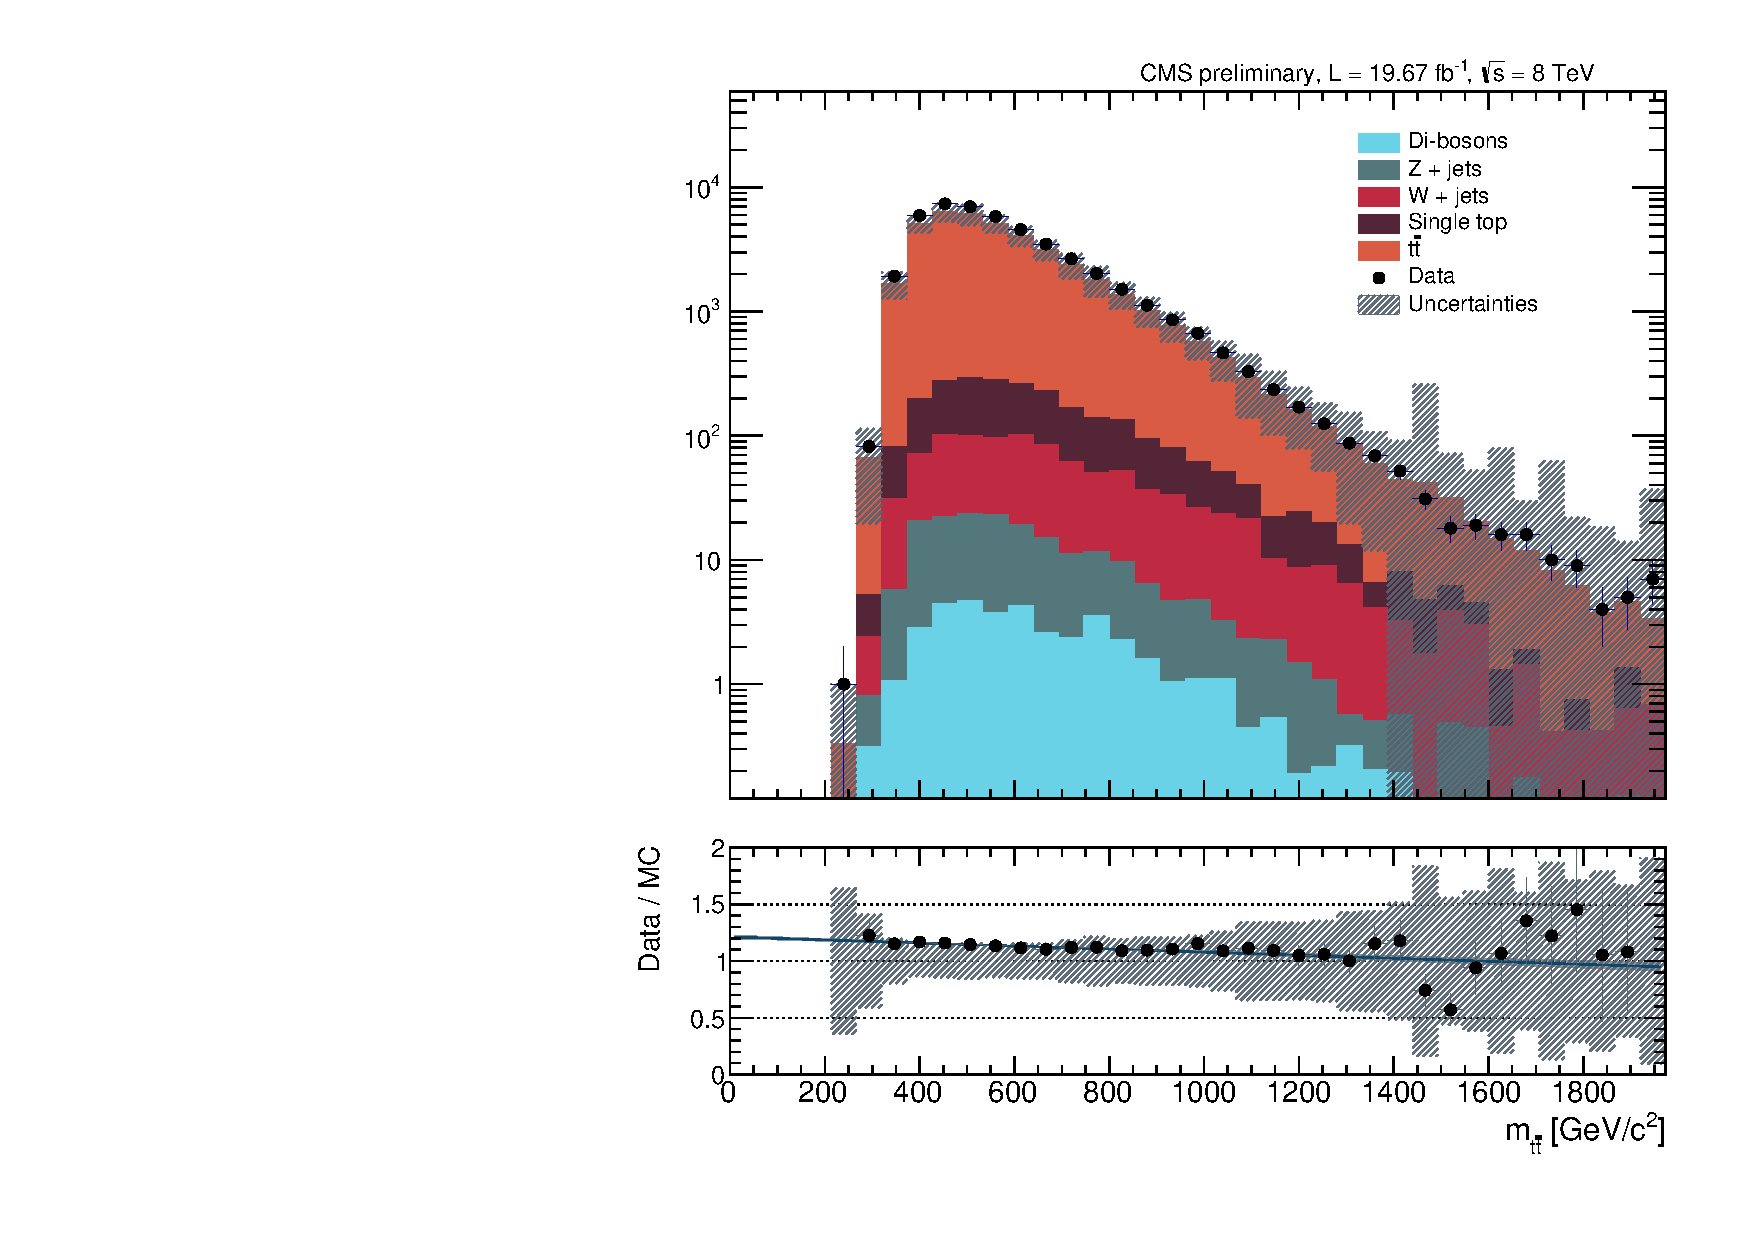
\includegraphics[width=0.49\textwidth,angle=-90,origin=c]{chapitre8/figs/data_mc_old_syst/2-btag/semie/mttSelected_btag_sel_reco_fullsel.pdf}}
%     \caption{Comparaison entre les données et la simulation, en sélectionnant au moins 2 jets étiquetés \Pbottom{}. Un ratio est présenté en bas de la distribution. La simulation est normalisée à la luminosité collectée, et la zone hachurée correspond aux incertitudes statistiques + systématiques.}
%     \label{fig:higgs_data_mc_2b}
% \end{figure}
%  \begin{figure}[p!] \centering
%     \subcaptionbox{Canal semi-muonique}[0.49\textwidth]{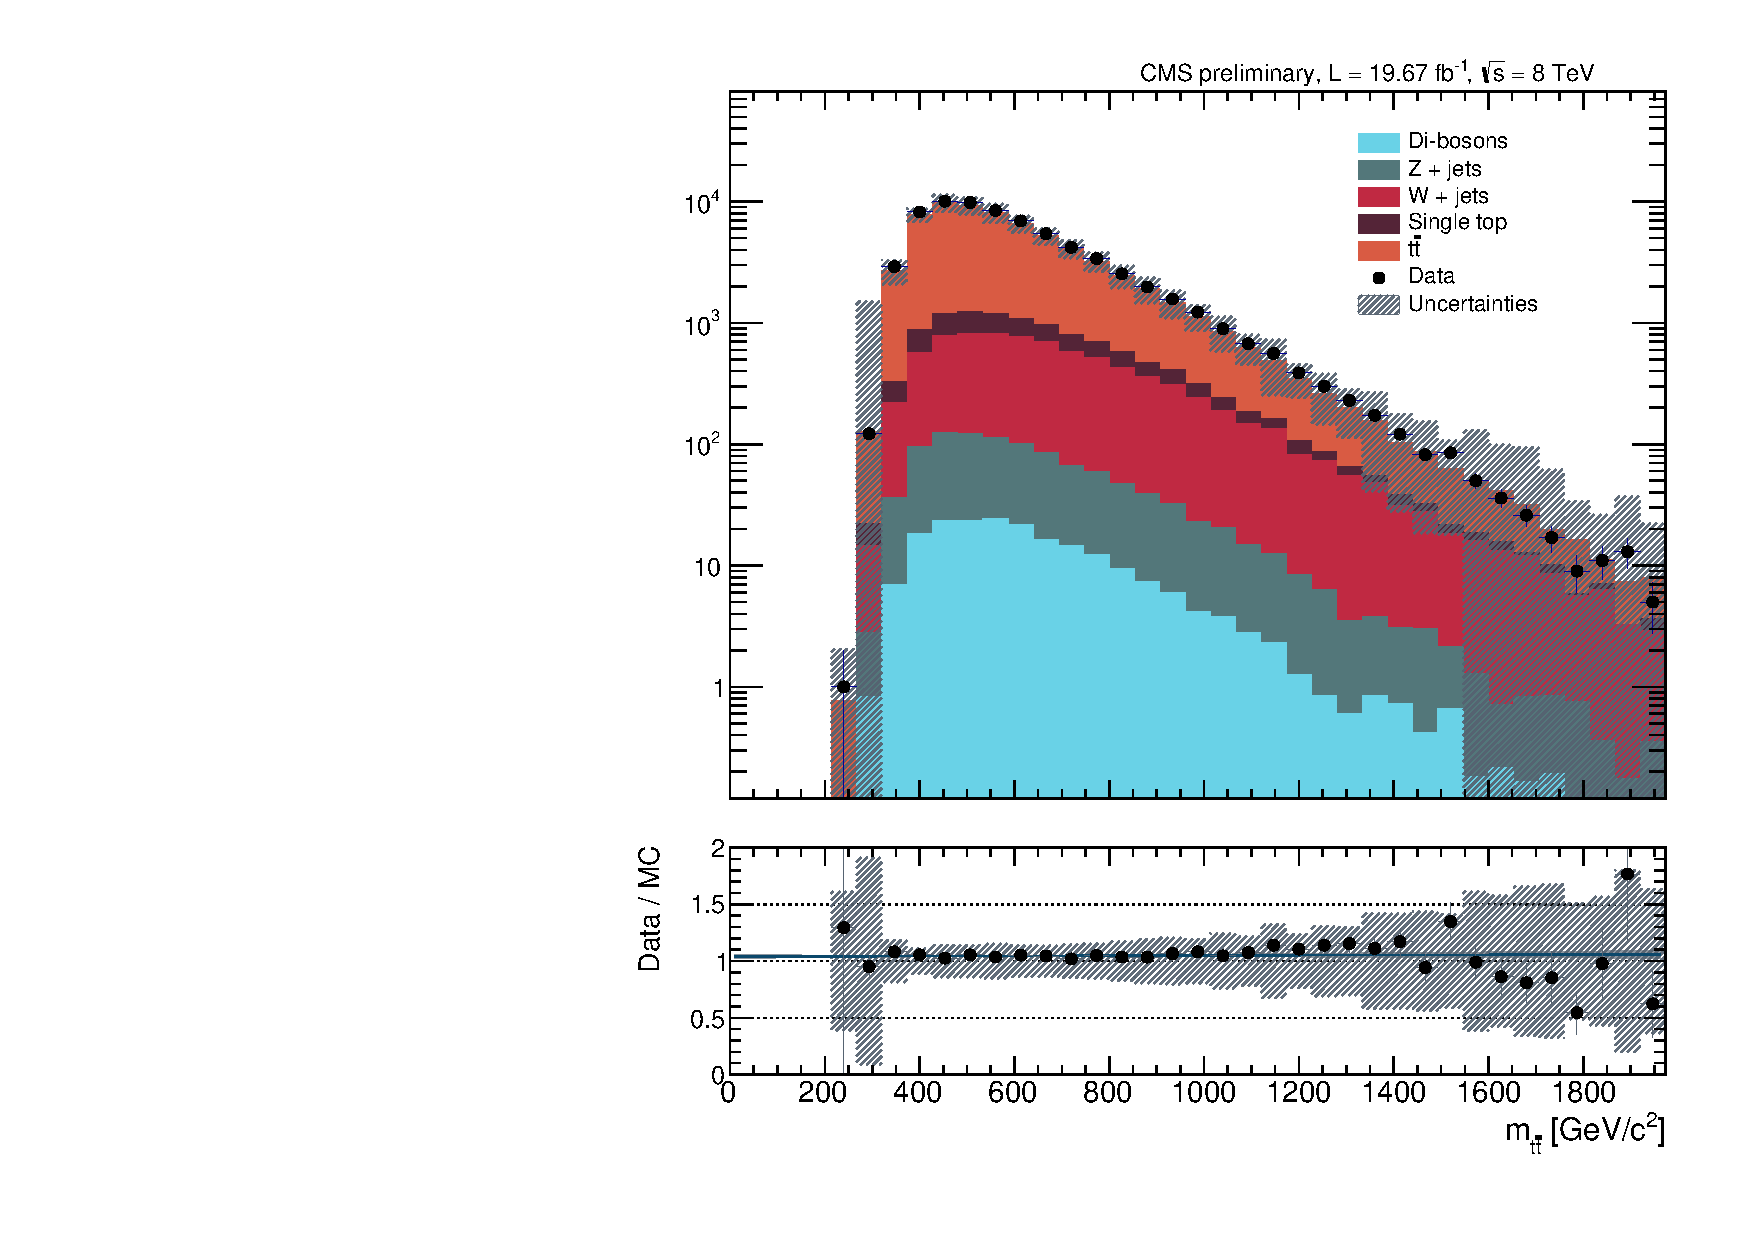
\includegraphics[width=0.49\textwidth,angle=-90,origin=c]{chapitre8/figs/data_mc_old_syst/1-btag/semimu/mttSelected_btag_sel_reco_fullsel.pdf}} \hfill
%     \subcaptionbox{Canal semi-électronique}[0.49\textwidth]{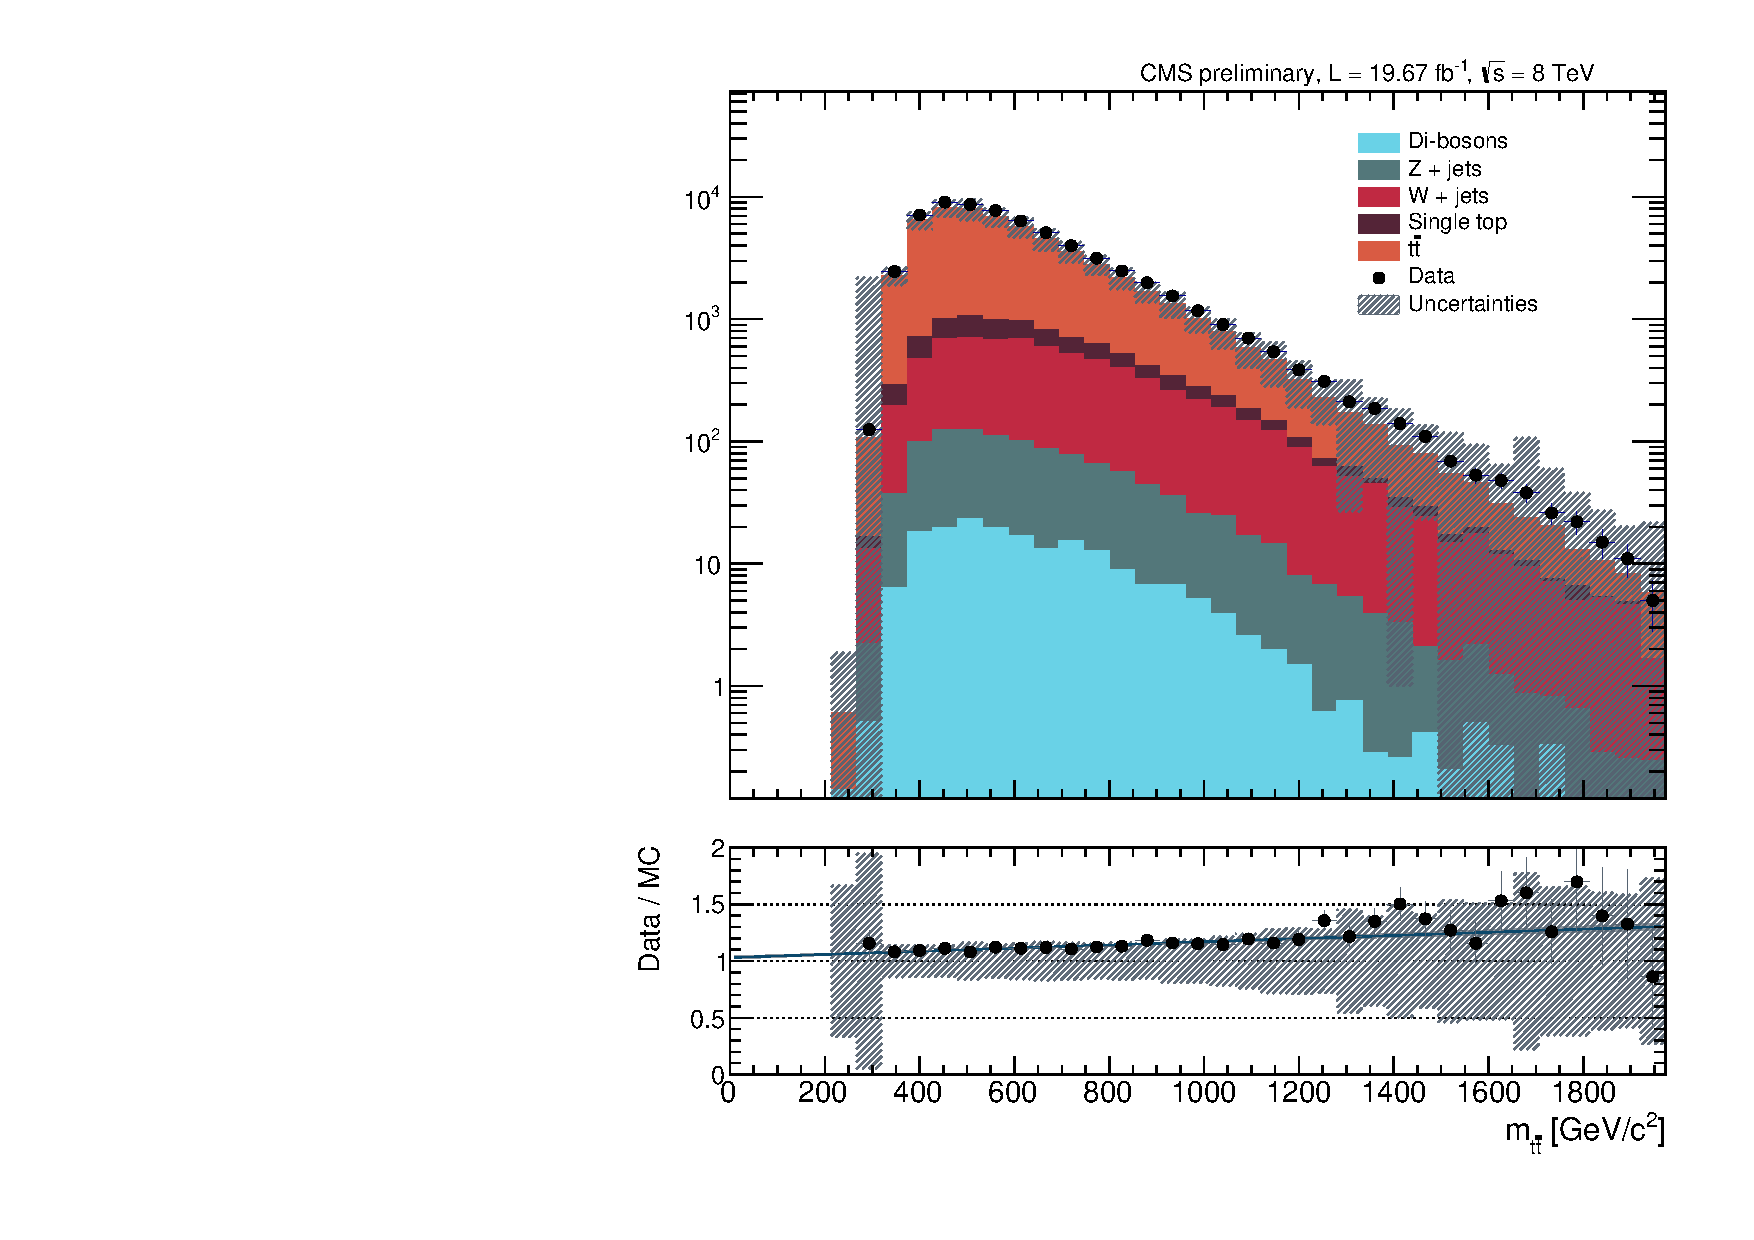
\includegraphics[width=0.49\textwidth,angle=-90,origin=c]{chapitre8/figs/data_mc_old_syst/1-btag/semie/mttSelected_btag_sel_reco_fullsel.pdf}}
%     \caption{Comparaison entre les données et la simulation, en sélectionnant exactement moins 1 jet étiqueté \Pbottom{}. Un ratio est présenté en bas de la distribution. La simulation est normalisée à la luminosité collectée, et la zone hachurée correspond aux incertitudes statistiques + systématiques.}
%     \label{fig:higgs_data_mc_1b}
% \end{figure}

\begin{figure}[p!] \centering
    \captionsetup{format=plain,indention=0.2cm,font=small,labelfont={sf,bf},justification=centering}
    \subcaptionbox{Canal semi-muonique,\\au moins 2 jets étiquetés \Pbottom}[0.49\textwidth]{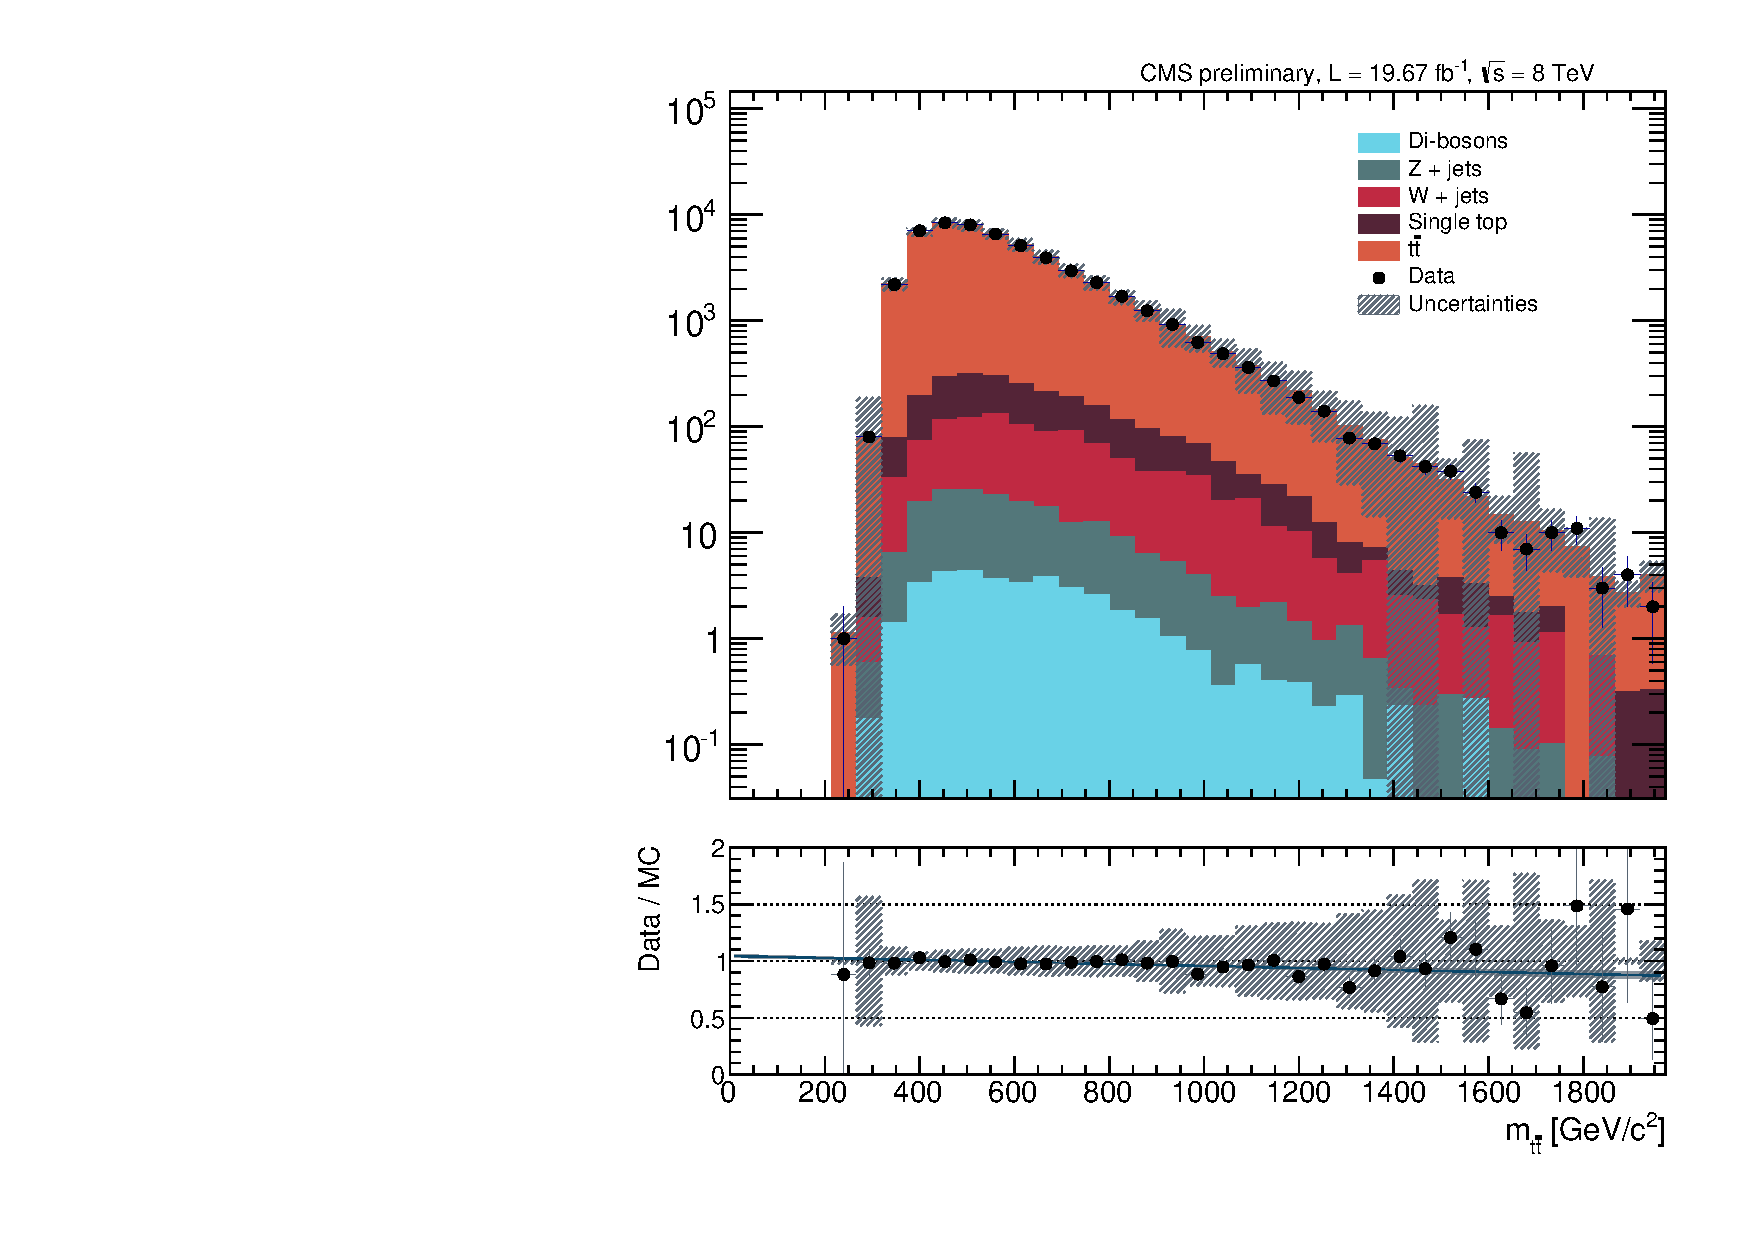
\includegraphics[width=0.49\textwidth,angle=-90,origin=c]{chapitre8/figs/data_mc/without_shift/2-btag/semimu/mttSelected_btag_sel_reco_fullsel.pdf}} \hfill
    \subcaptionbox{Canal semi-électronique,\\au moins 2 jets étiquetés \Pbottom}[0.49\textwidth]{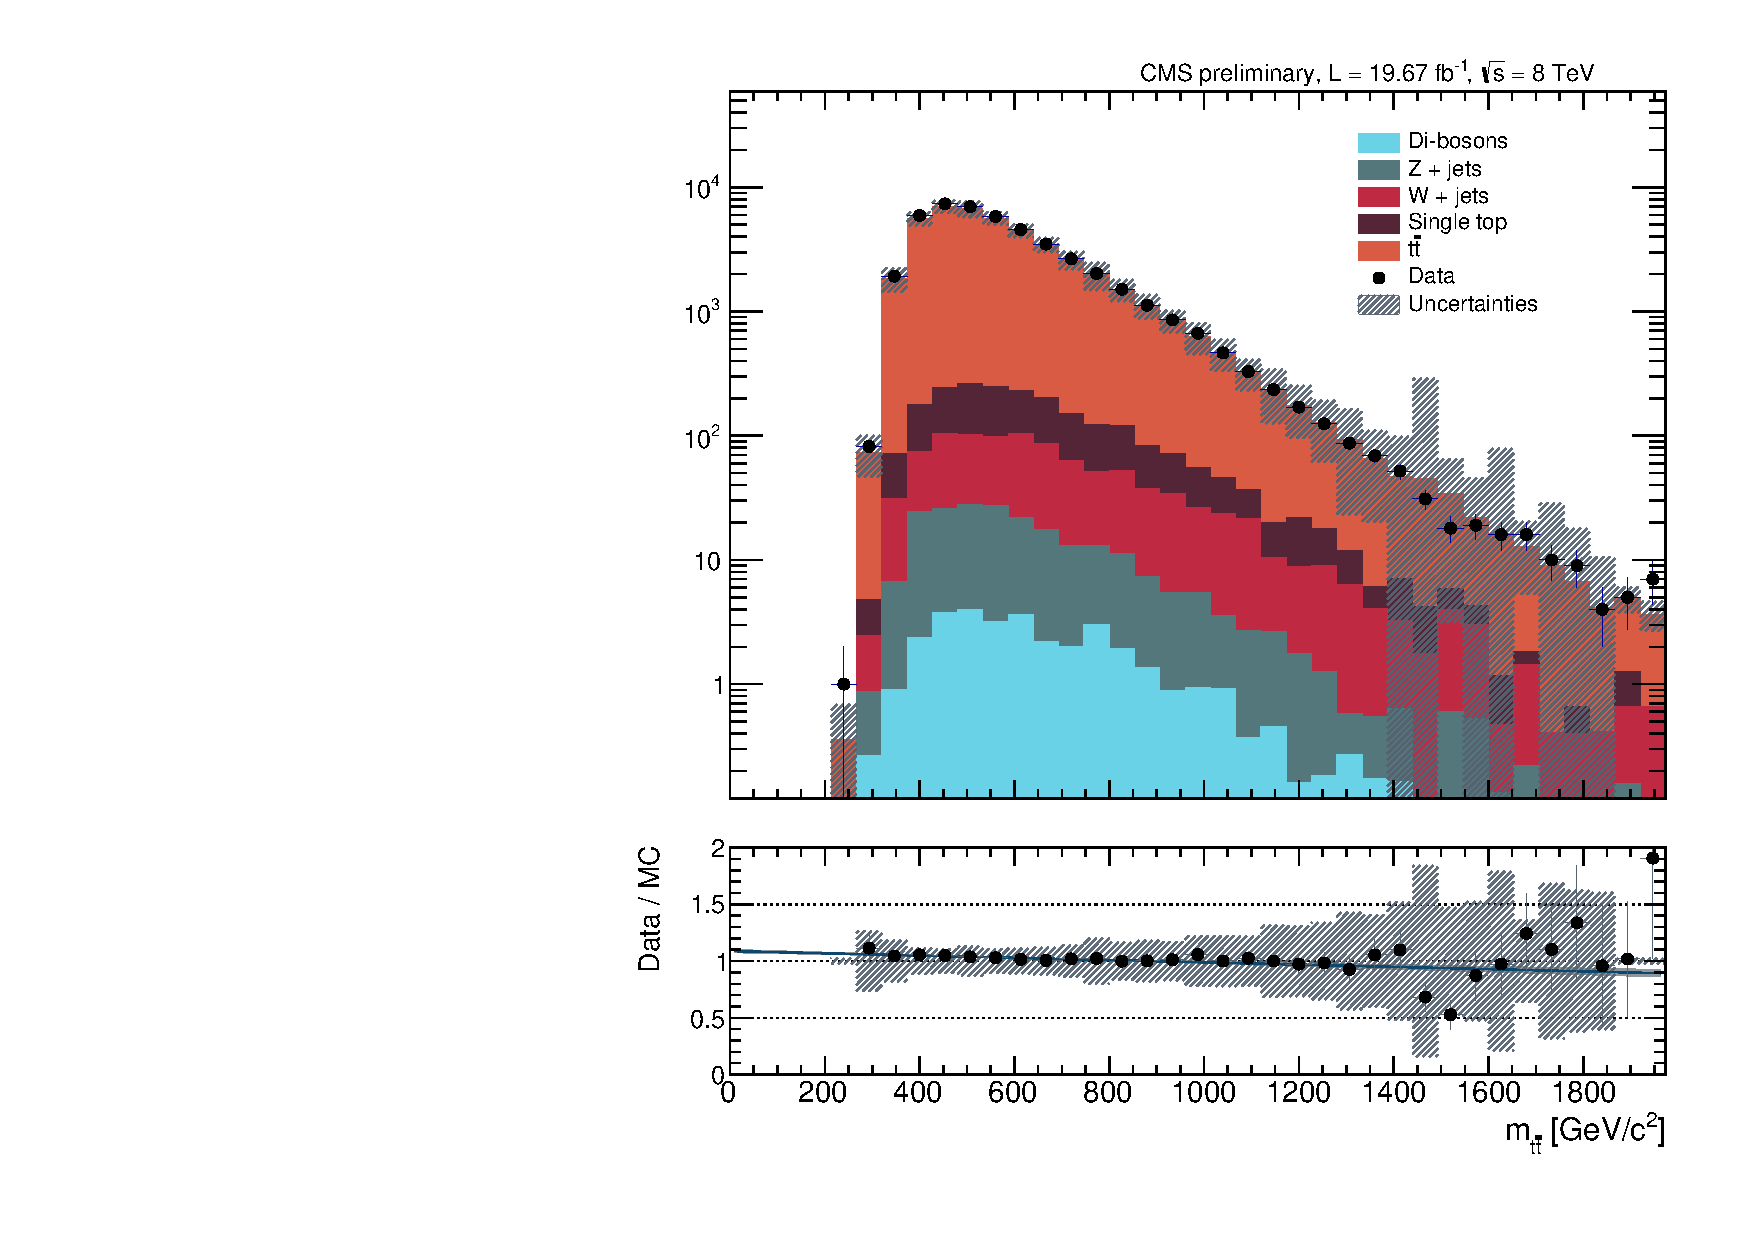
\includegraphics[width=0.49\textwidth,angle=-90,origin=c]{chapitre8/figs/data_mc/without_shift/2-btag/semie/mttSelected_btag_sel_reco_fullsel.pdf}} \\ \vspace{5mm}
    \subcaptionbox{Canal semi-muonique,\\exactement 1 jet étiqueté \Pbottom}[0.49\textwidth]{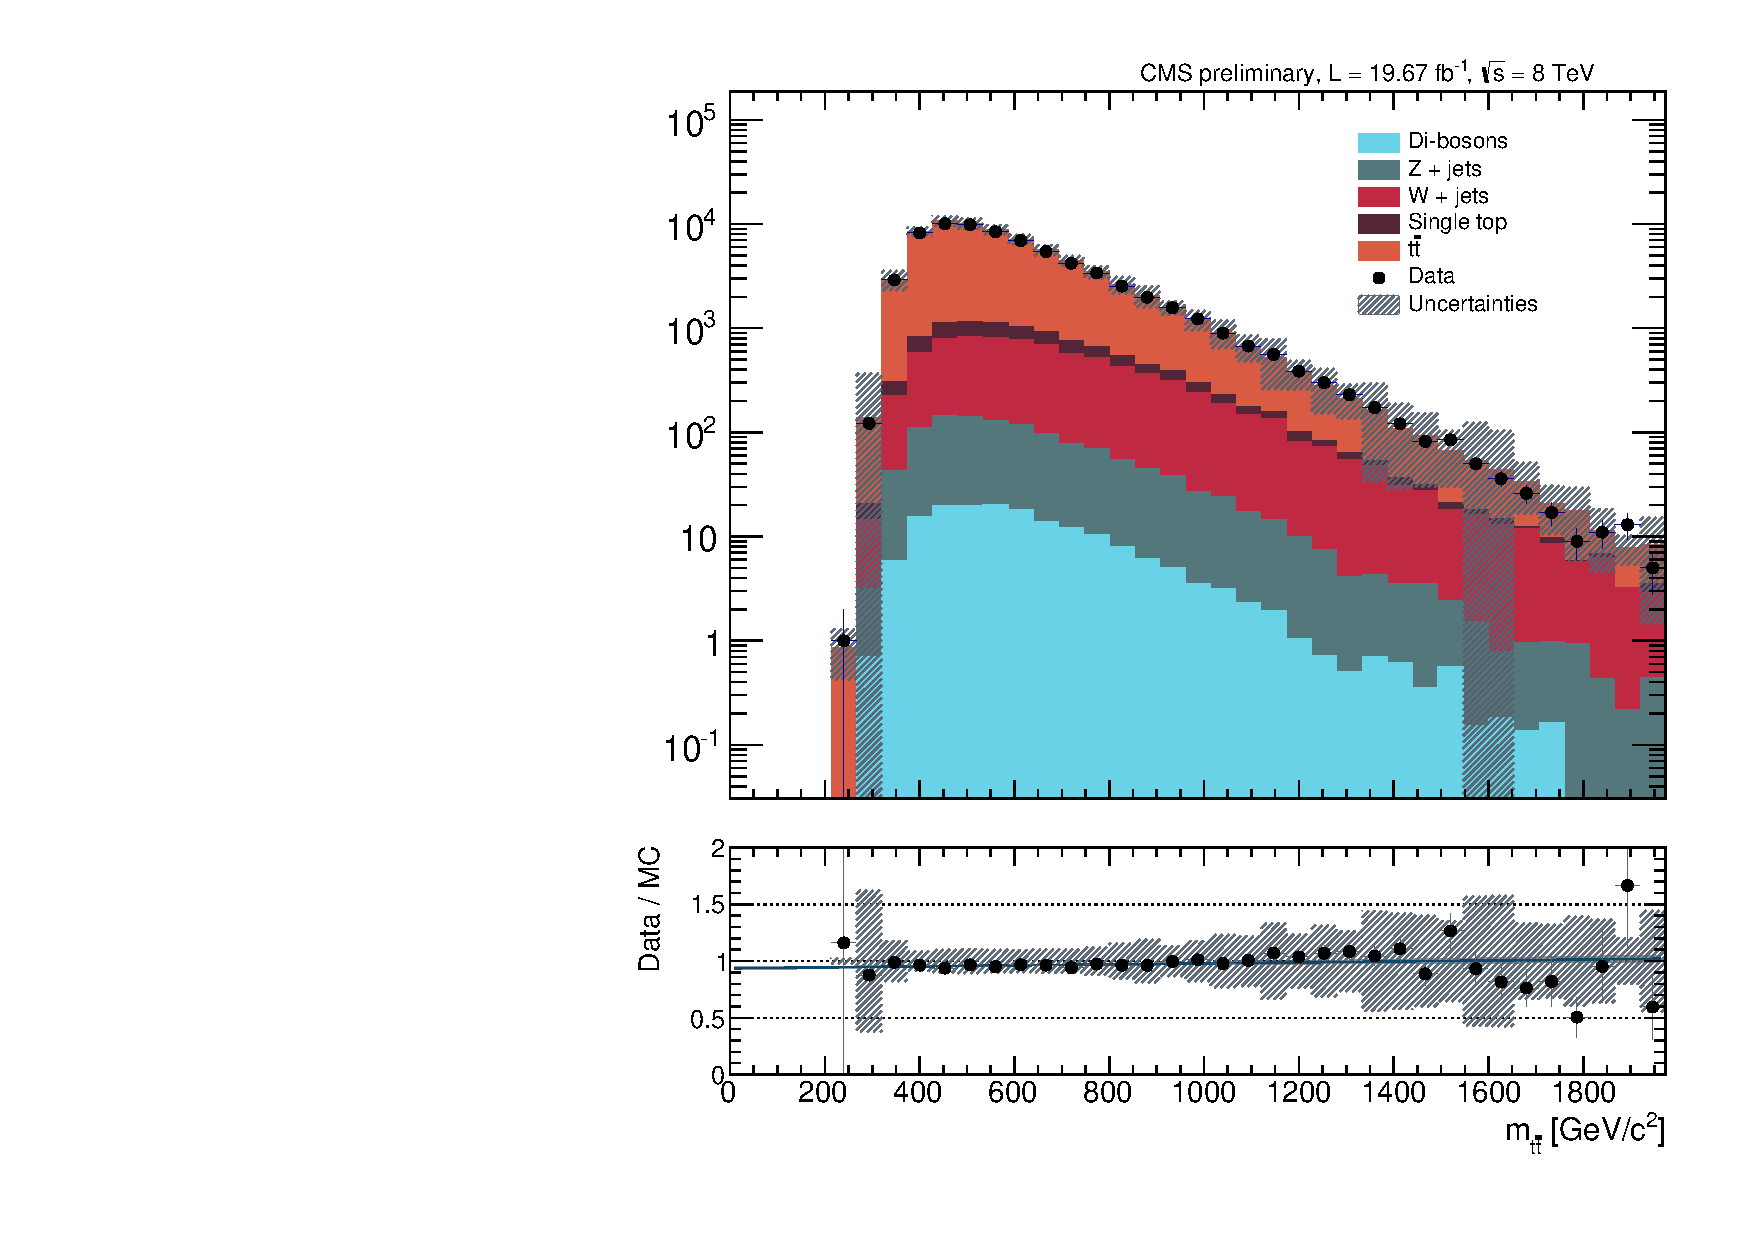
\includegraphics[width=0.49\textwidth,angle=-90,origin=c]{chapitre8/figs/data_mc/without_shift/1-btag/semimu/mttSelected_btag_sel_reco_fullsel.pdf}} \hfill
    \subcaptionbox{Canal semi-électronique,\\exactement 1 jet étiqueté \Pbottom}[0.49\textwidth]{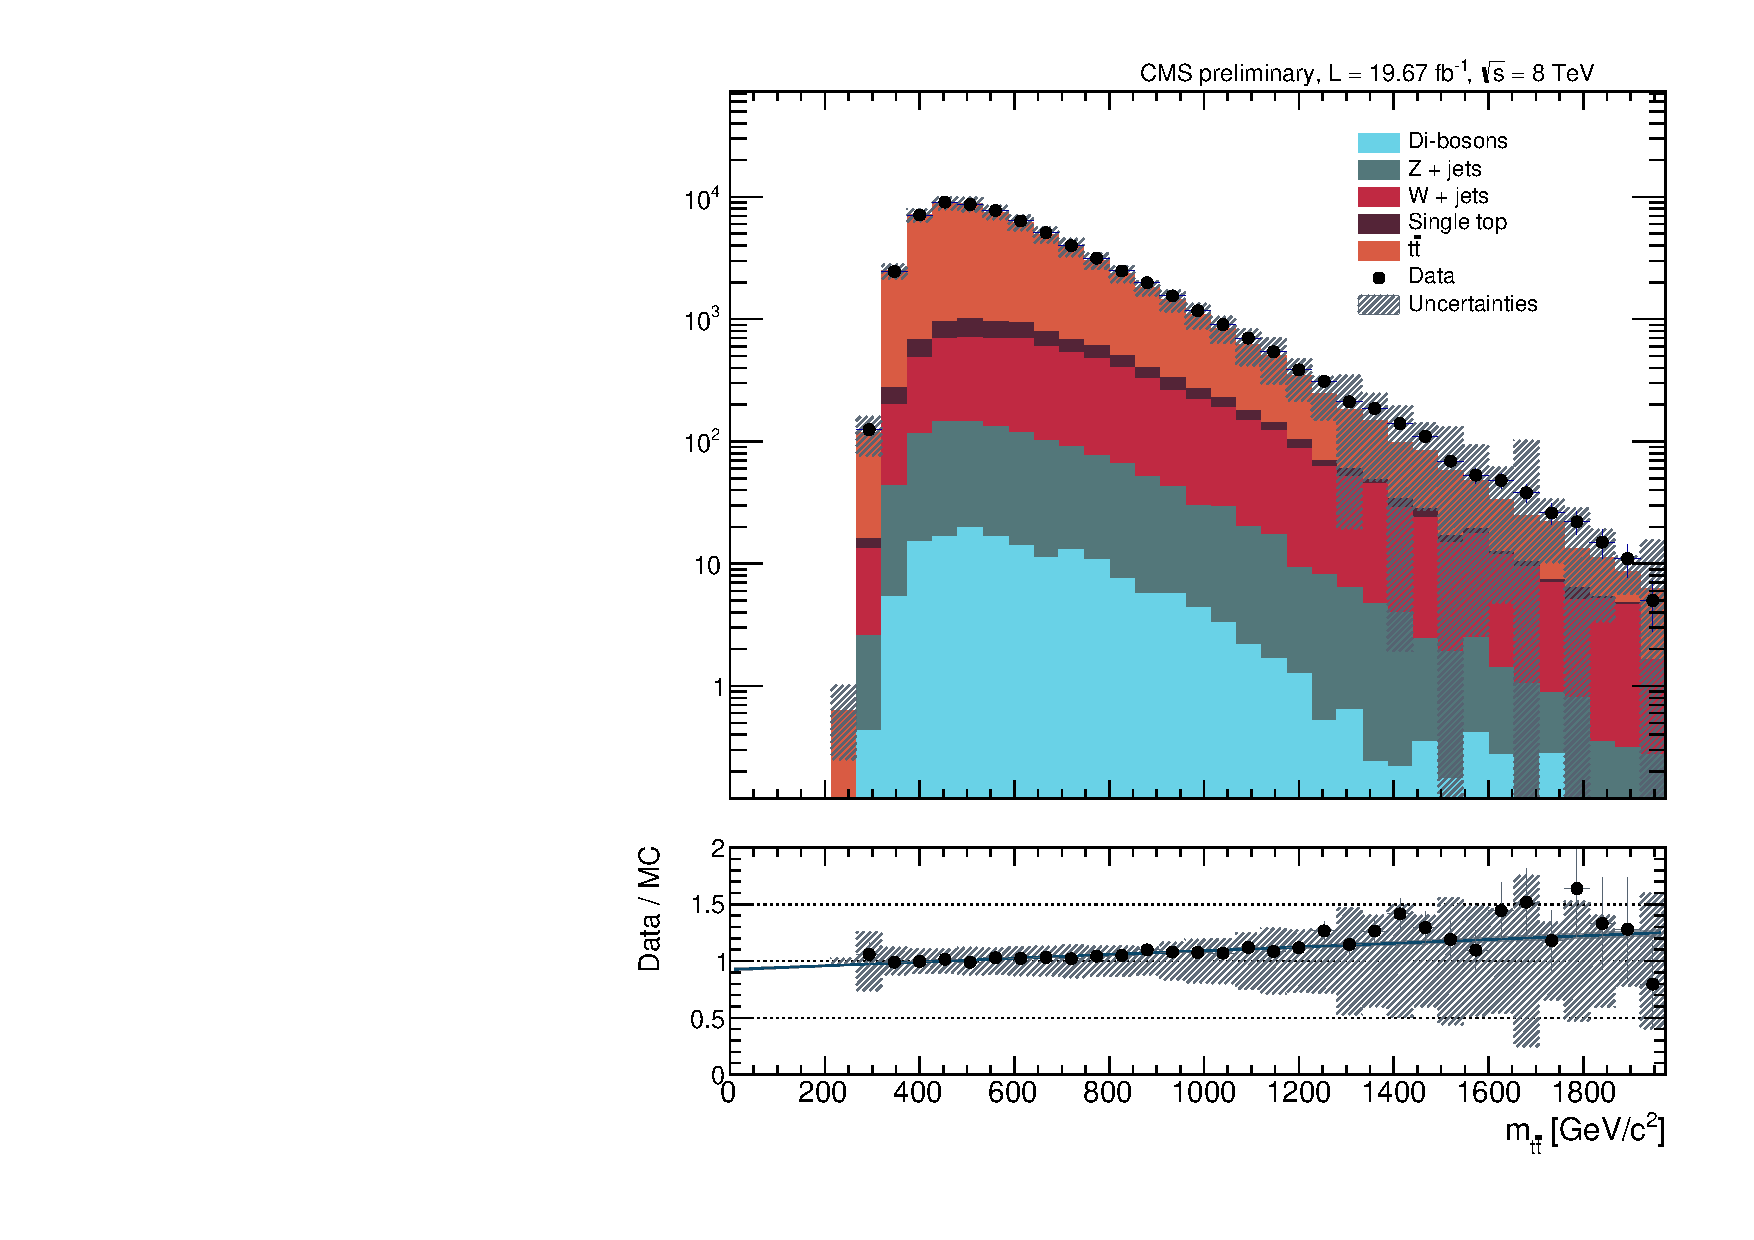
\includegraphics[width=0.49\textwidth,angle=-90,origin=c]{chapitre8/figs/data_mc/without_shift/1-btag/semie/mttSelected_btag_sel_reco_fullsel.pdf}}
    \captionsetup{format=plain,indention=0.2cm,font=small,labelfont={sf,bf},justification=justified}
    \caption{Comparaison entre les données et la simulation. Un ratio est présenté en bas de la distribution. La simulation est normalisée aux valeurs de sorties d'un ajustement sur les données par la méthode du maximum de vraisemblance. La zone hachurée correspond aux incertitudes statistiques + systématiques.}
    \label{fig:higgs_data_mc}
\end{figure}

\begin{table} \centering% \sisetup{separate-uncertainty = true} \small
\begin{tabular}{ccccc} \toprule
 & \multicolumn{2}{c}{semi-$\mu$} & \multicolumn{2}{c}{semi-e} \\ \cmidrule{2-5}
 & $N_{\Pbottom} == 1$ & $N_{\Pbottom} \geq 2$  & $N_{\Pbottom} == 1$ & $N_{\Pbottom} \geq 1$ \\ \midrule
 \ttbar & \num{61881.73} & \num{50626.43} & \num{53021.79} & \num{42605.62} \\
 Top célibataire & \num{2625,65} & \num{1479,12} & \num{2200,39} & \num{1237,9} \\
 \PW + jets & \num{6704,42} & \num{884,17} & \num{5777,97} & \num{731,86} \\
 \PZ + jets & \num{1014,09} & \num{162,87} & \num{1093,29} & \num{187,85} \\
 Di-bosons & \num{169,94} & \num{38,33} & \num{154,35} & \num{32,29} \\ \cmidrule{1-1}
 Total & \num{72396 \pm 9260} & \num{53191 \pm 7669} & \num{62248 \pm 8794} & \num{44796 \pm 6756} \\ \cmidrule{1-1}
 Données & \num{69862} & \num{52885} & \num{63892} & \num{46184} \\
 \bottomrule
\end{tabular}
\caption{Nombre d’événements attendus et observés après sélection pour une luminosité de \SI{19,7}{\invfb}, après application des facteurs de corrections extraient de l'ajustement par la méthode du maximum de vraisemblance. L'incertitude sur le nombre d'événements attendus tient compte des incertitudes statistiques et systématiques. Le nombre d'événements attendus est différent du nombre d'événements observés puisque l'ajustement est réalisé simultanément sur les 4 catégories de l'analyse.}
\label{tab:higgs_yield}
\end{table}

Le \cref{tab:higgs_yield} résume le nombre d'événements attendus et observés pour une luminosité intégrée de \SI{19.7}{\invfb}, après application des facteurs de corrections extraits de l'ajustement par la méthode du maximum de vraisemblance. L'incertitude sur le nombre d'événements attendus tient compte des incertitudes statistiques et systématiques. Le nombre d'événements attendus et observés est différent puisque l'ajustement est réalisé simultanément sur les 4 catégories de l'analyse. On constate cependant que le nombre d'événements observés est compatible avec les prédictions théoriques dans les incertitudes systématiques, et ce pour toutes les catégories.

\begin{table} \centering% \sisetup{separate-uncertainty = true} \small
\begin{tabular}{cc} \toprule
  & Facteur de correction \\ \midrule
 \ttbar & \num{1.11} \\
 Top célibataire & \num{0.79} \\
 \PW + jets & \num{1.23} \\
 \PZ + jets & \num{0.97} \\
 Di-bosons & \num{0.84} \\
 \bottomrule
\end{tabular}
\caption{Facteurs de corrections extraits d'un ajustement simultané des 4 catégories de l'analyse sur les données, par la méthode du maximum de vraisemblance.}
\label{tab:higgs_corr}
\end{table}

\section{Analyse statistique} \label{sec:higgs_stat}

Le nombre d'événements dans chaque classe de \mtt suit une loi de Poisson de moyenne $\lambda_i$. On définit ainsi la fonction de vraisemblance $\mathcal{L}$ comme le produit des lois de Poisson pour chaque classe :
\begin{align*}
  \mathcal{L} &= \prod\limits_{i = 0}^B \left( \frac{\lambda_i^{n_i} \, e^{- \lambda_i}}{n_i!} \right) \\
\end{align*}
où $B$ est le nombre de classes de \mtt et $n_i$ le nombre d'événements observés dans la classe $i$. $\lambda_i$, le nombre d'événements attendus dans la classe $i$, est défini par
\begin{align*}
  \lambda_i &= \mu S_i + \sum \limits_k B_{k, i}
\end{align*}
Ici, $k$ court sur tous les bruits de fonds considérés, $B_{k, i}$ est le nombre d'événements du bruit de fond $k$ dans la classe $i$, $S_i$ le nombre d'événements de signal dans la classe $i$ et $\mu$ l'intensité du signal. Le signal est normalisé à la luminosité collectée ainsi qu'à la section efficace de production à l'arbre prédite par \texttt{MadGraph}.

\medskip

La présence d'incertitudes systématiques impacte le nombre d'événements attendus $\lambda_i$. Un paramètre de nuisance est ajouté à la fonction de vraisemblance pour chaque source d'incertitude systématique. Pour les paramètres de nuisances impactant seulement la normalisation, un coefficient est ajouté avec un \emph{prior} log-normal. Pour les paramètres impactant à la fois la forme et la normalisation, un coefficient est ajouté avec un \emph{prior} gaussien : la valeur de ce coefficient est utilisée afin d'interpoler la forme de la distribution entre la forme nominale et les formes obtenues en appliquant une variation de $\pm 1 \sigma$ sur le paramètre d'intérêt de l'incertitude systématique.

\section{Incertitudes systématiques} \label{sec:higgs_syst}

Plusieurs sources d'incertitudes sont considérées, listées ci-dessous. Il est important de noter que ces incertitudes affectent à la fois les distributions du signal et des bruits de fond. Pour chaque source, les distributions de signal et de bruit de fond sont déterminées à nouveau et l'effet propagé au résultat.

\begin{description}
  \item[Luminosité] L'incertitude sur la mesure de la luminosité (\SI{2.6}{\percent}) est considérée comme une source d'incertitude systématique, impactant la normalisation des échantillons.
  \item[\pu] La section efficace des collisions \Pproton{}\Pproton{} utilisée lors du calcul des facteurs de repondération du \pu est variée de \pm{} \SI{5}{\percent}. La variation de la forme des distribution est considérée comme une source d'incertitude, impactant la forme et la normalisation des échantillons.
  \item[Facteurs de corrections] Les incertitudes sur les facteurs de corrections liés à l'identification et à l'isolation des leptons, à l'algorithme d'étiquetage des jets de \Pbottom ainsi qu'aux performances des chemins de déclenchement sont considérées comme des sources d'incertitudes systématiques, impactant la forme et la normalisation des échantillons.
  \item[Corrections des jets] Les incertitudes sur les corrections en énergie et résolution des jets sont considérées comme une source d'incertitudes systématiques, impactant la forme et la normalisation des échantillons.
  \item[Sections efficaces des bruits de fonds] Afin de prendre en compte les incertitudes systématiques sur la normalisation des bruits de fonds, on introduit une incertitude systématique impactant uniquement la normalisation des échantillons. Cette incertitude est de \SI{15}{\percent} pour \ttbar, \SI{30}{\percent} pour le bruit de fond top célibataire, et \SI{50}{\percent} pour \PW + jets, \PZ + jets et di-bosons.
  \item[Modélisation des bruits de fonds] Une variation simultanée des échelles de factorisation et de renormalisation d'un facteur \num{0.5} et \num{2} est utilisée afin d'estimer les incertitudes liées à l'absence d'ordres supérieurs dans la simulation Monte-Carlo des bruits de fonds \ttbar, \PW + jets et \PZ + jets.
\end{description}

\section{Résultats}

En cas d'absence d'interférences entre le signal et le bruit de fond, le nombre d'événements de signal est directement proportionnel à sa section efficace de production. Cette relation de proportionnalité est utilisée lors de la procédure d'extraction des limites, où le nombre d'événements de signal est ajusté sur les données et converti en limite supérieure sur la section efficace.
La présence d'interférences ne permet plus d'établir une relation de proportionnalité simple entre le nombre d'événements et la section efficace théorique. En effet, la section efficace est donnée schématiquement par
\begin{align*}
  \sigma_\text{S + I} &= \sigma - \sigma_\text{\ttbar} \propto \mathcal{M}_\text{S}^2 + \mathcal{M}_\text{S}^\ast \mathcal{M}_\text{B} + \mathcal{M}_\text{S} \mathcal{M}_\text{B}^\ast
\end{align*}
\begin{figure}[tbp] \centering
    \subcaptionbox{Scalaire, $\sz = \SI{500}{\GeV}$}[0.48\textwidth]{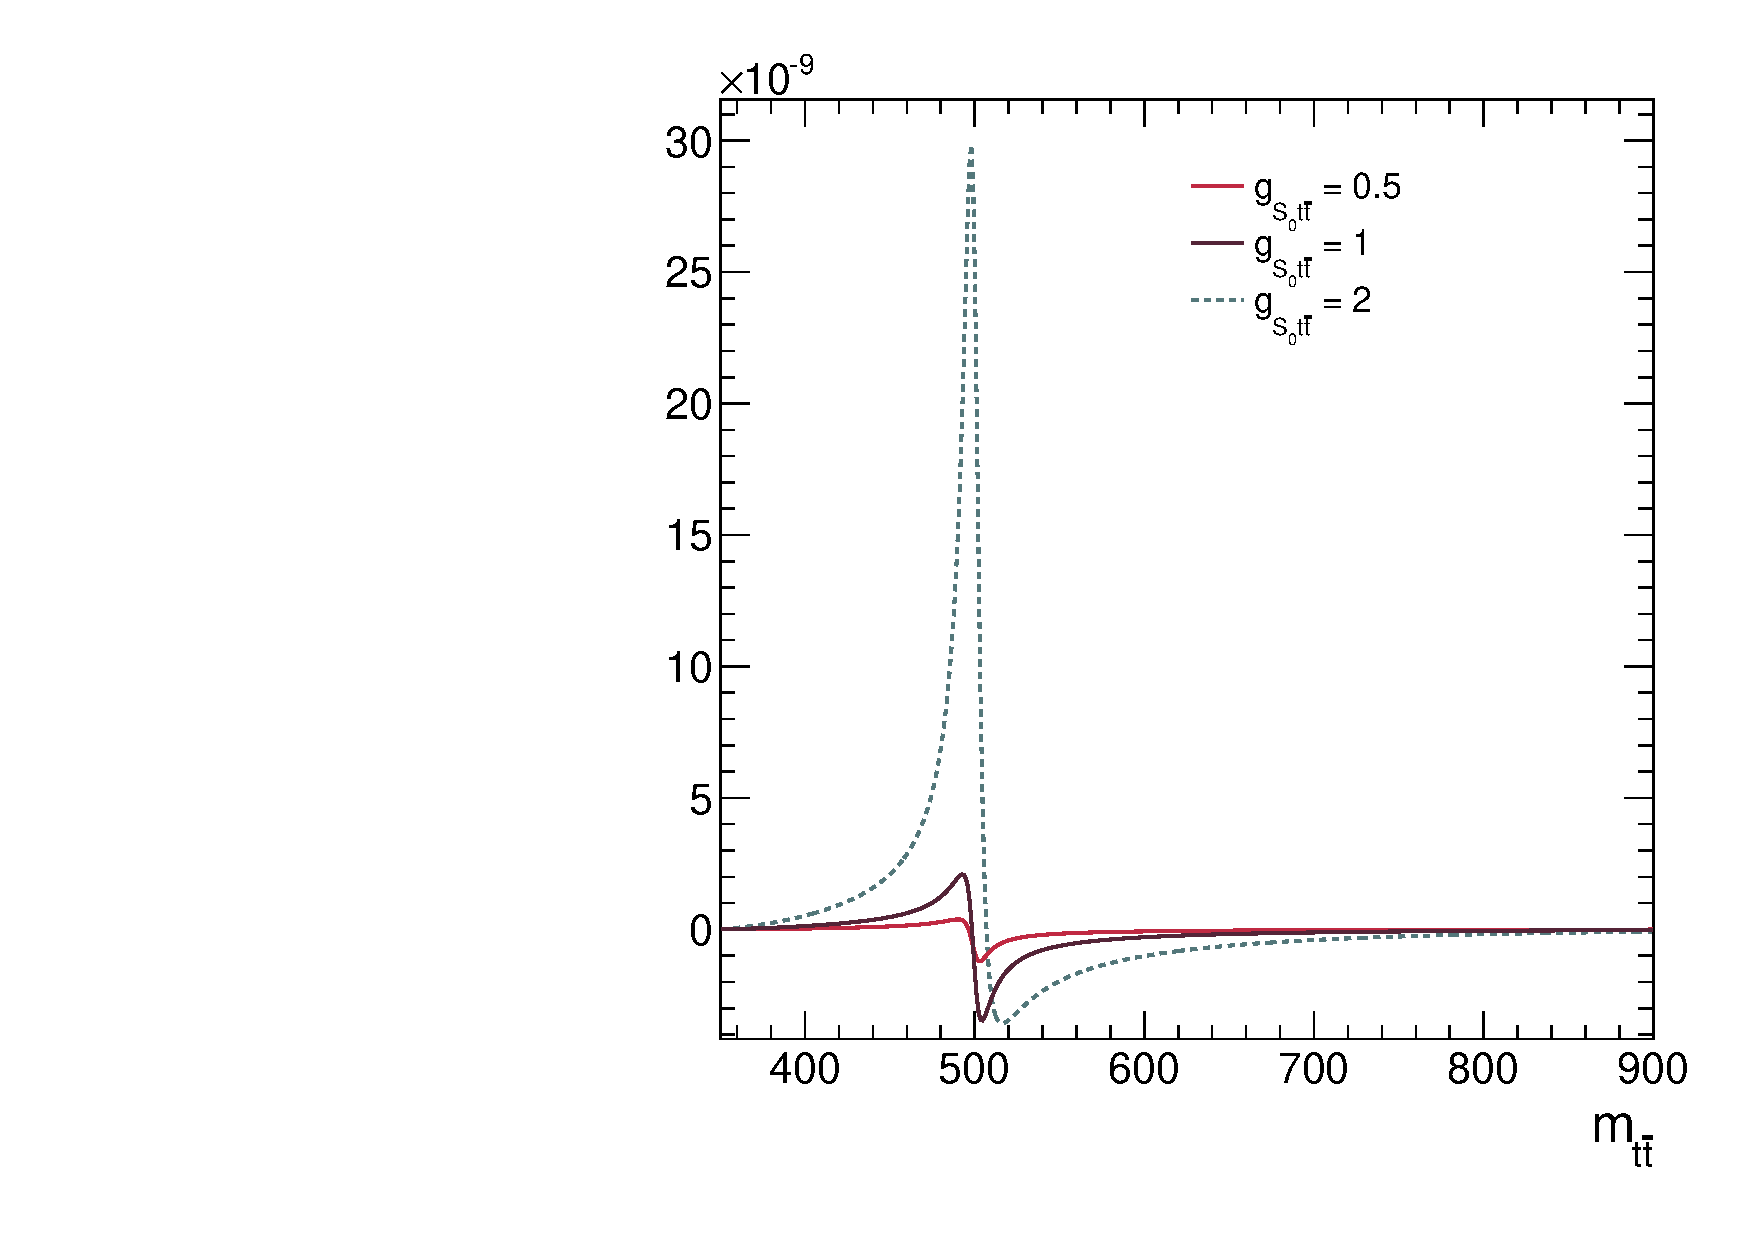
\includegraphics[width=0.48\textwidth,angle=-90,origin=c]{chapitre8/figs/S0/scalar_int_various_couplings.pdf}}
    \subcaptionbox{Pseudo-scalaire, $\sz = \SI{500}{\GeV}$}[0.48\textwidth]{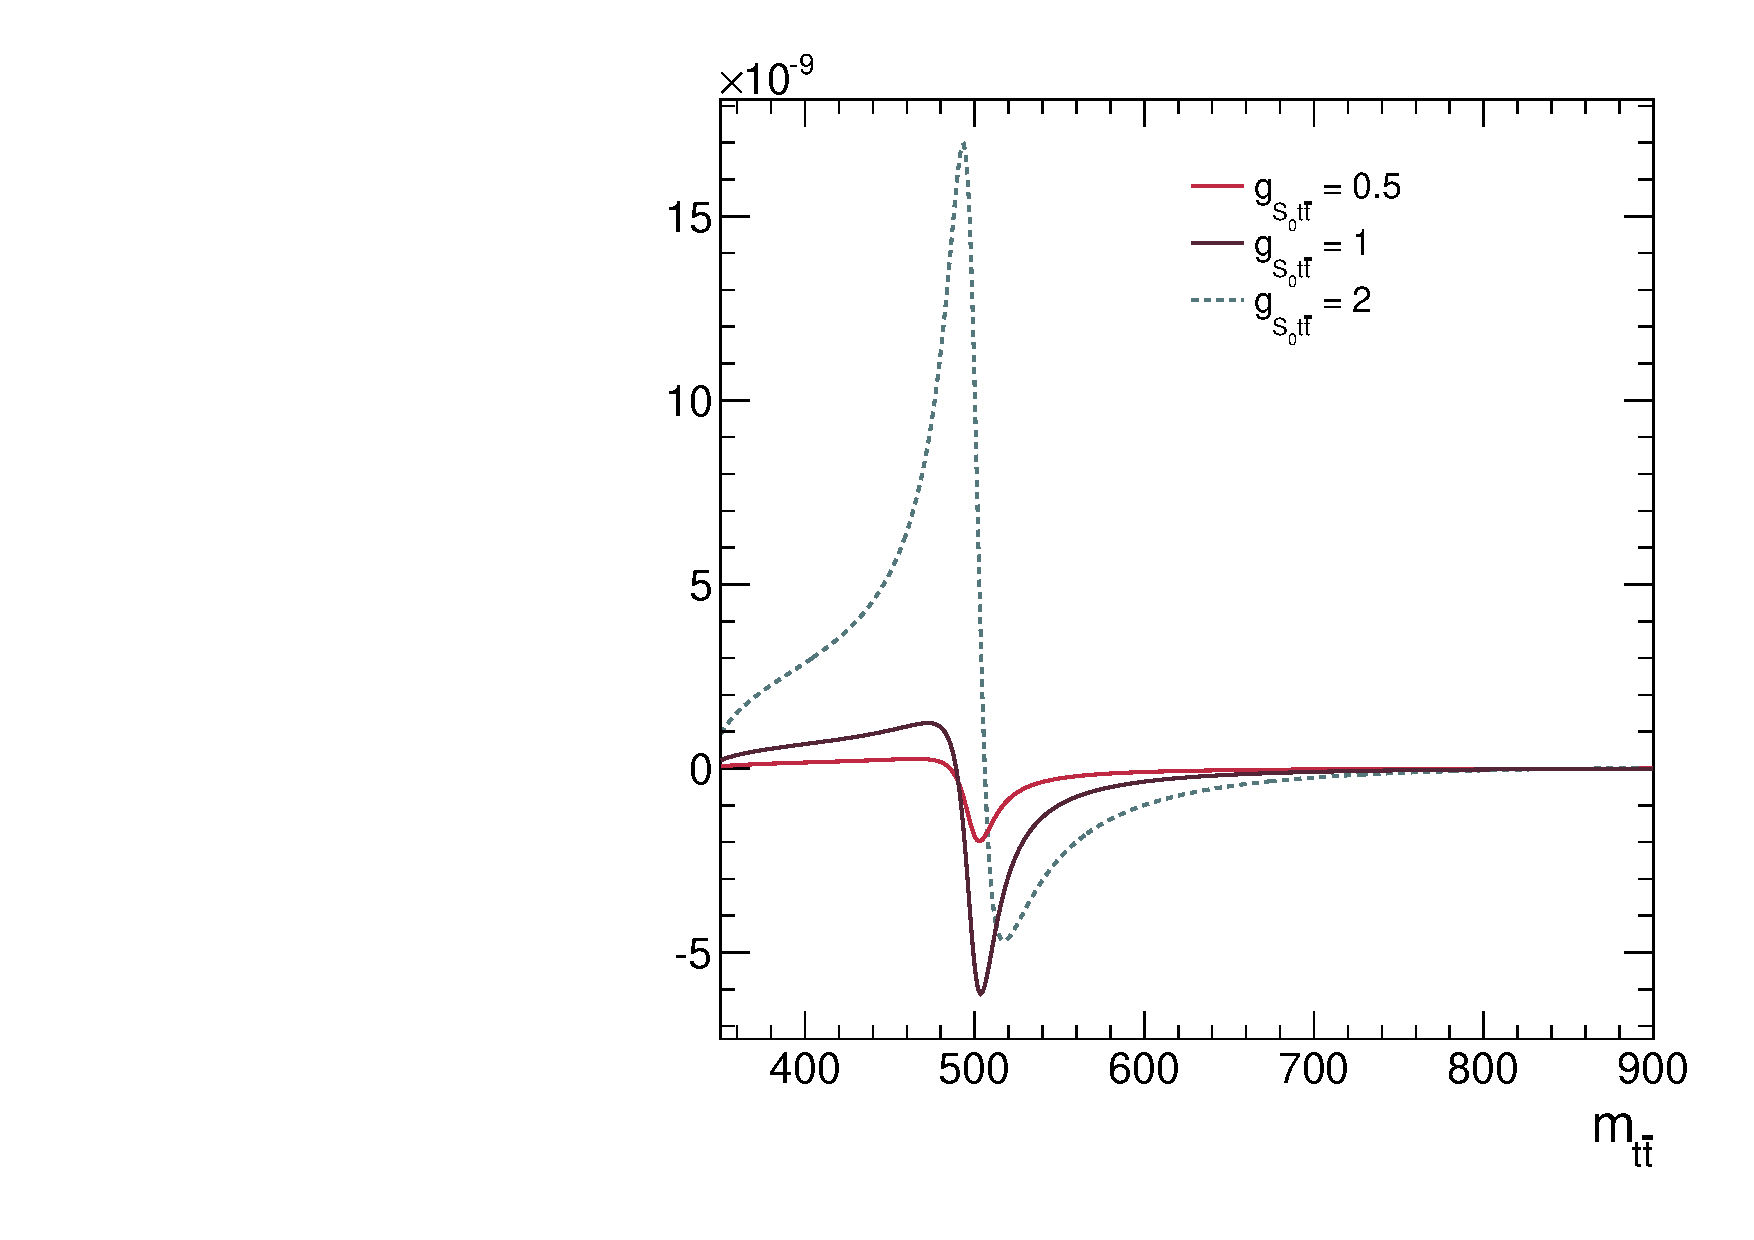
\includegraphics[width=0.48\textwidth,angle=-90,origin=c]{chapitre8/figs/S0/pseudoscalar_int_various_couplings.pdf}}
    \caption{Effet de la valeur du couplage $g_{\sz \ttbar}$ sur la forme de la distribution de masse invariante, pour un \sz de masse $\msz = \SI{500}{\GeV}$.}
    \label{fig:sig_coupling}
\end{figure}
où $\mathcal{M}_\text{S}$ est proportionnel à $g_{\sz \ttbar}^4$, alors que $\mathcal{M}_\text{S} \mathcal{M}_\text{B}$ est proportionnel à $g_{\sz \ttbar}^2$. Ainsi, changer la section efficace revient à changer le couplage entre \sz et \ttbar, ce qui impacte directement la structure de l'interférence. En effet, en modifiant $g_{\sz \ttbar}$, la section efficace du signal et celle de l'interférence ne sont pas modifiées d'un facteur identique, modifiant la forme de la distribution de masse invariante (voir \cref{fig:signal_interference}). Cette forme est donc fixée par la section efficace, et change de façon non prévisible lorsque la section efficace change. L'effet d'un changement de couplage entre \sz et \ttbar est visible sur la \cref{fig:sig_coupling}, pour un \sz de masse $\msz = \SI{500}{\GeV}$. Comme on peut le voir, le ratio entre l'excès et le déficit change en fonction du couplage. Il n'est ainsi pas possible de laisser le nombre d'événements de signal varier lors de l'ajustement sur les données.

\medskip

Le but de cette analyse est donc d'évaluer la compatibilité des données observées avec une hypothèse de signal dans laquelle la section efficace est fixée. À terme, une analyse plus complète pourrait contraindre l'espace des paramètres pour ce type de modèles. Cela demande des simulations dédiées aussi pour différentes valeurs de couplages.

\bigskip

Afin de quantifier la sensibilité de l'analyse à un possible signal de nouvelle physique, on utilise une approche fréquentiste, qui permet de déterminer la probabilité que les données collectées soient compatibles avec une hypothèse d'absence de signal (\emph{p-value}). On définit pour cela un test statistique $q$, basé sur un rapport de fonctions de vraisemblance. On a
\begin{align*}
  q &= \log{ \frac{\mathcal{L}_\text{s + b}}{\mathcal{L}_\text{b}} }
\end{align*}
où $\mathcal{L}_\text{s + b}$ est la fonction de vraisemblance dans l'hypothèse de la présence de signal ($\mu = 1$), et $\mathcal{L}_\text{b}$ est la fonction de vraisemblance dans l'hypothèse d'absence de signal ($\mu = 0$). Chaque fonction de vraisemblance est maximisée avant l'évaluation de $q$.

\medskip

On extrait dans un premier temps la valeur attendue de $q$, $q_0$. Pour cela, \num{20000} pseudo\-/expériences sont générées à partir de la simulation, dans l'hypothèse de présence de signal. Pour chaque pseudo\-/expérience, le test statistique $q$ est calculé. On obtient ainsi une distribution, de laquelle on extrait $q_0$, défini comme la médiane de la distribution, ainsi que les intervalles de confiance à \SI{68}{\percent} et \SI{95}{\percent}, obtenus en intégrant respectivement \SI{68}{\percent} et \SI{95}{\percent} de la distribution autour de la médiane. Un exemple d'un telle distribution est présenté sur la \cref{fig:qzero} pour un \sz pseudo\-/scalaire de masse $\msz = \SI{500}{\GeV}$. La ligne bleue correspond à $q_0$, médiane de la distribution, la zone en vert foncé (vert clair) correspond à l'intervalle de confiance à \SI{68}{\percent} (\SI{95}{\percent}).

\begin{figure}[p!]
    \centering
    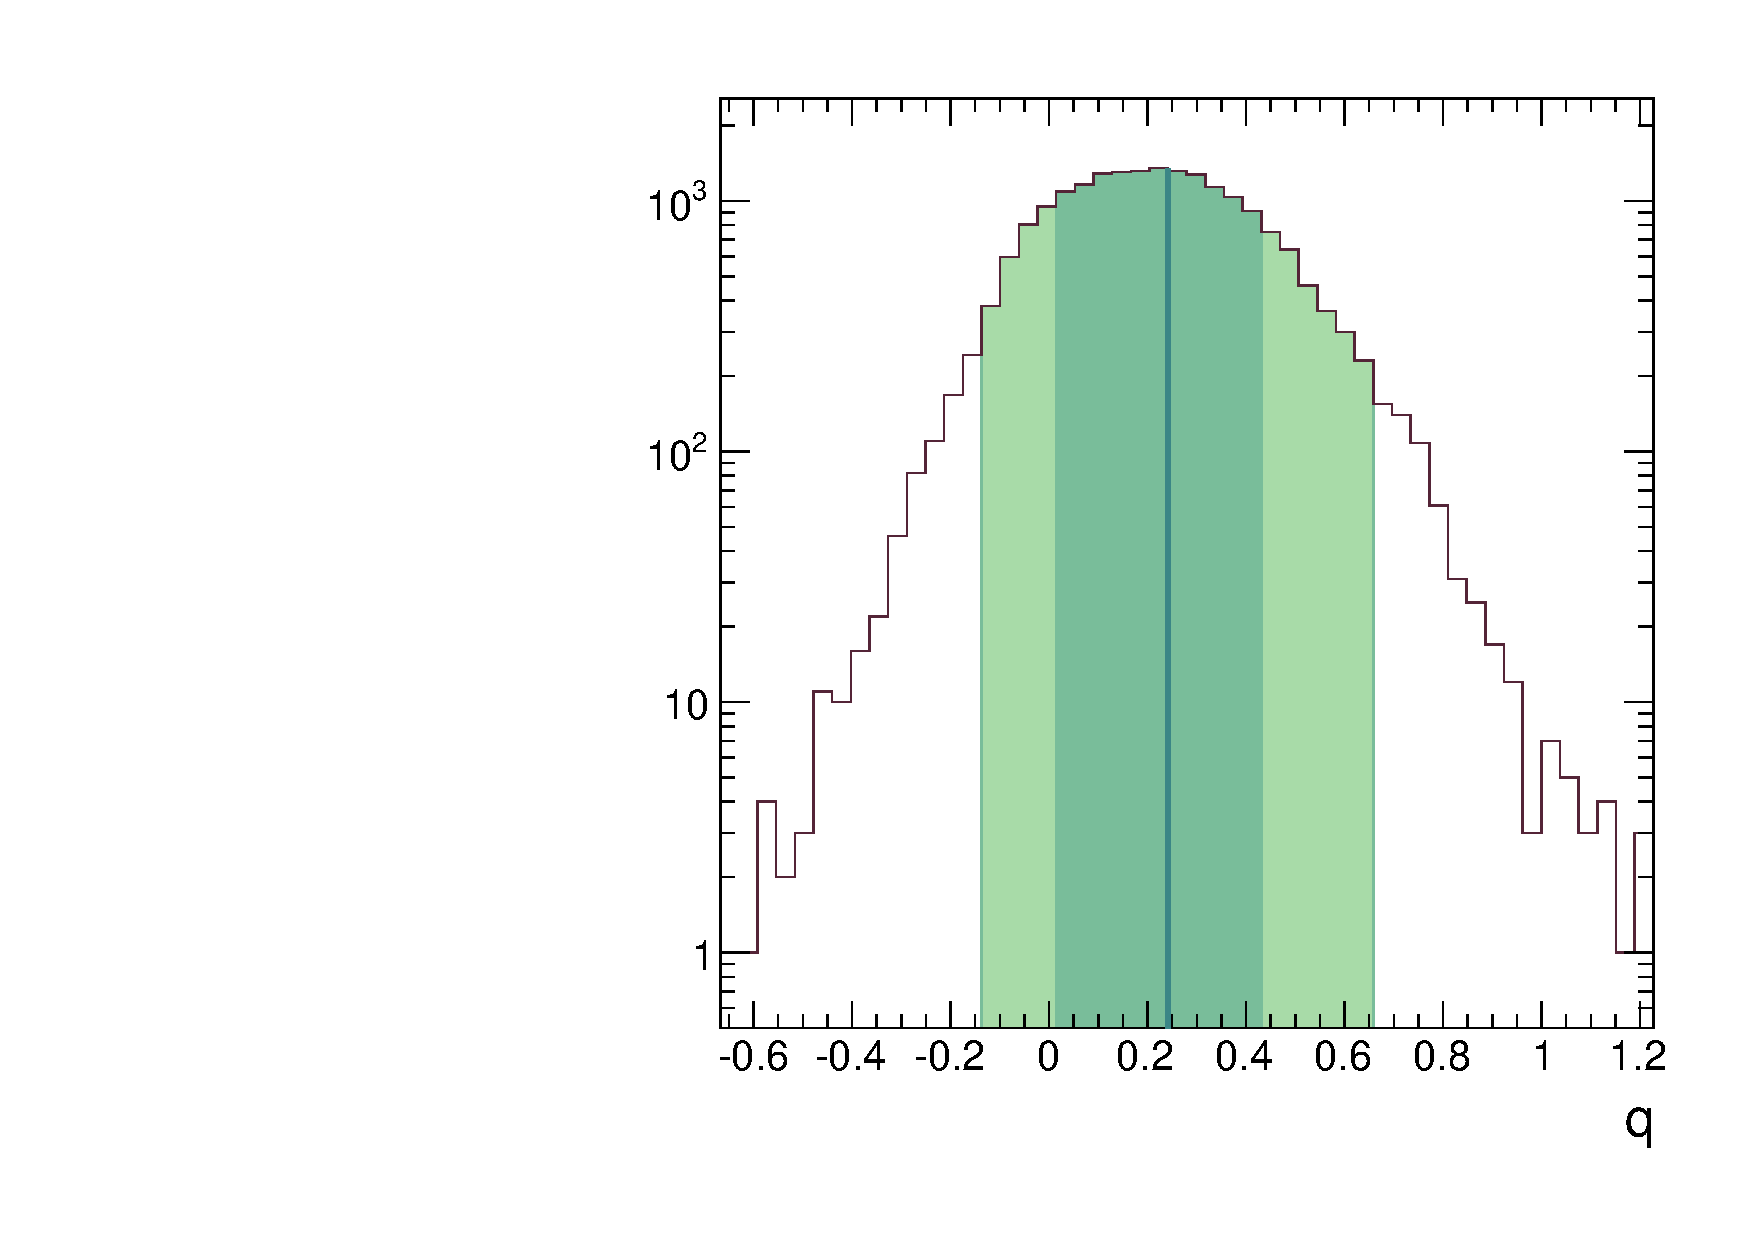
\includegraphics[width=0.6\textwidth,angle=-90,origin=c]{chapitre8/figs/stats/dnll_expected.pdf}
    \caption{Extraction de $q_0$ pour un \sz pseudo\-/scalaire de masse $\msz = \SI{500}{\GeV}$. La ligne bleue correspond à $q_0$, médiane de la distribution, la zone en vert foncé (vert clair) correspond à l'intervalle de confiance à \SI{68}{\percent} (\SI{95}{\percent}).}
    \label{fig:qzero}

    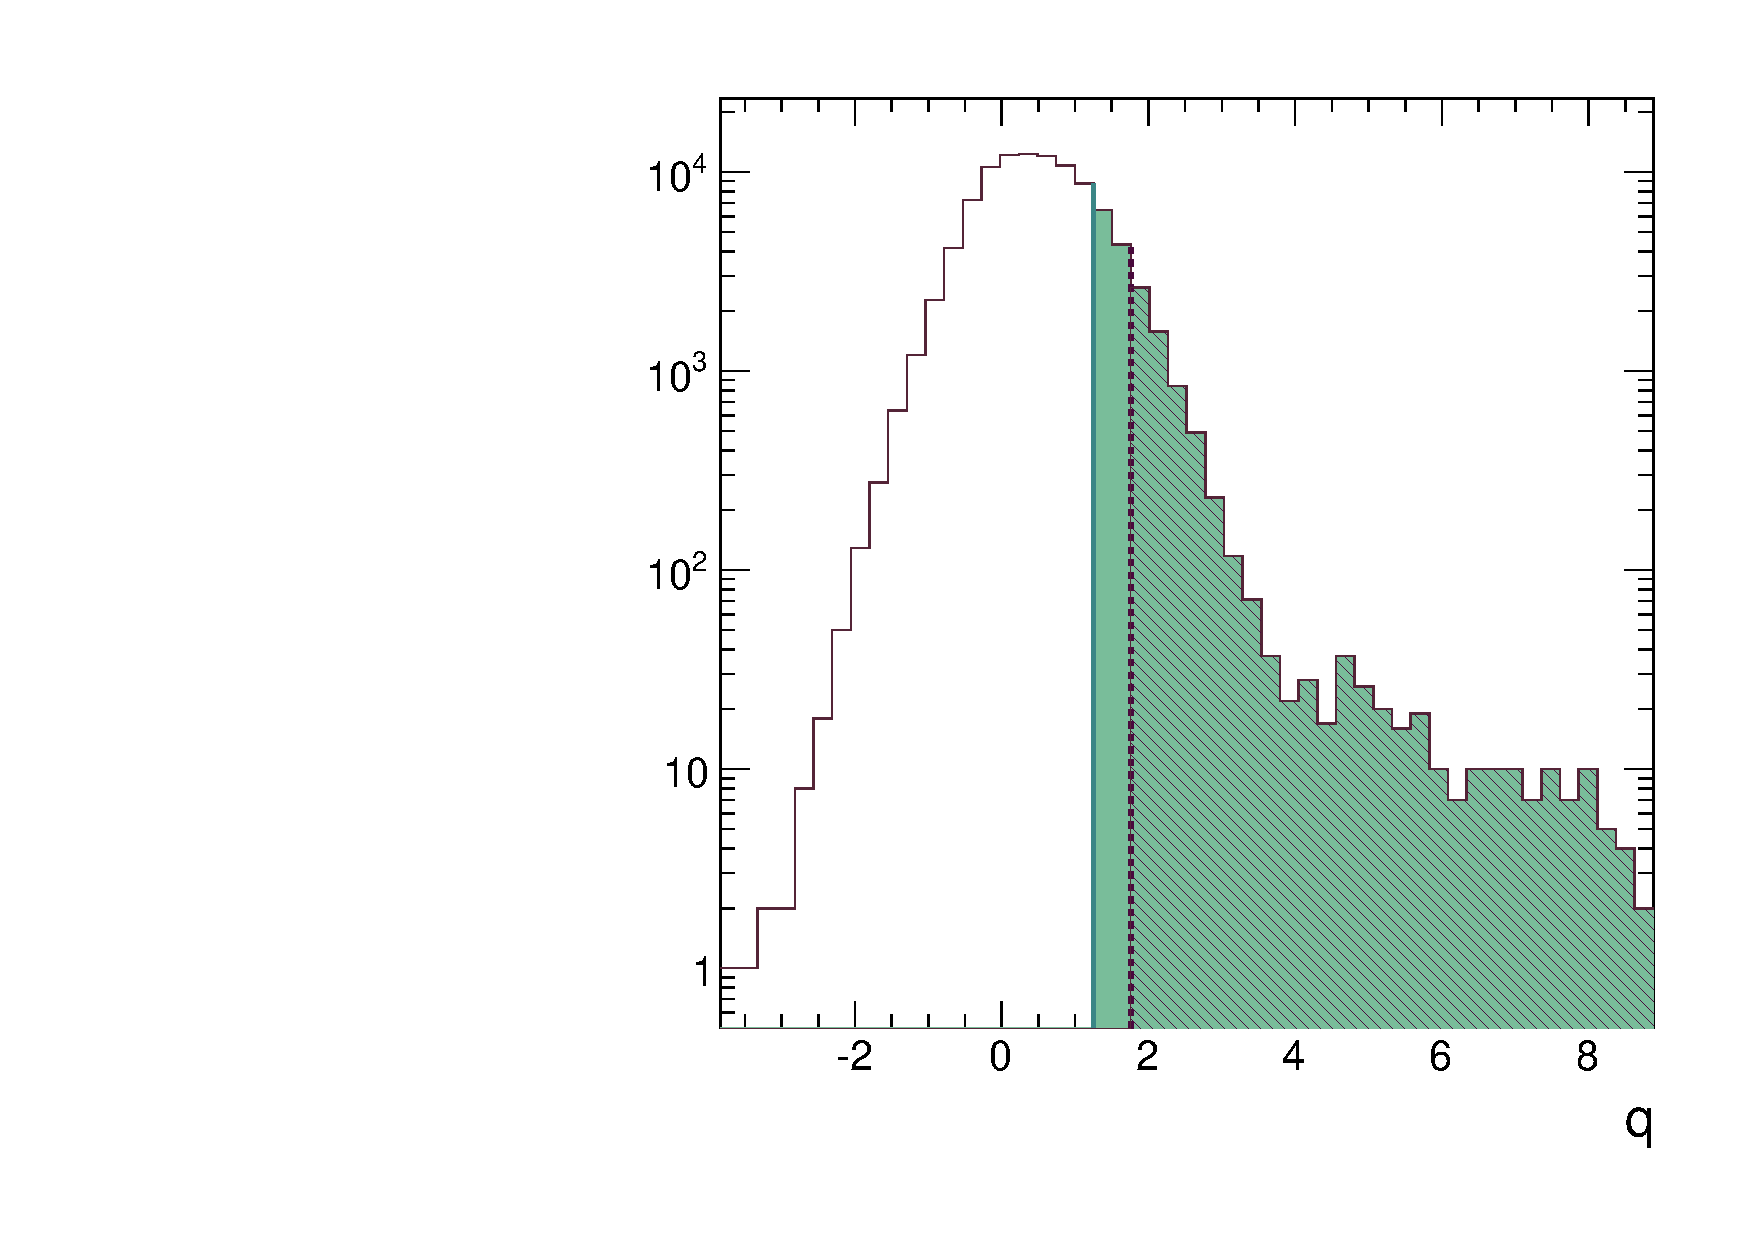
\includegraphics[width=0.6\textwidth,angle=-90,origin=c]{chapitre8/figs/stats/dnll_toy.pdf}
    \caption{Extraction de la \pvalue attendue pour un \sz pseudo\-/scalaire de masse $\msz = \SI{500}{\GeV}$. La ligne bleue correspond à $q_0$, la ligne pointillée violette à $q_\text{obs}$ et les zones vertes et hachurée représentent respectivement l'intégrale de la distribution à partir de $q_0$ et à partir de $q_\text{obs}$.}
    \label{fig:pvalues}
\end{figure}

La valeur observée $q_\text{obs}$ est extraite en calculant le test statistique $q$ sur les données.

\medskip

Afin de calculer la \emph{p-value} attendue et observée, \SI{100 000} pseudo-expériences sont générées dans l'hypothèse d'absence de signal. On obtient ainsi une nouvelle distribution $f(q)$. On définit la \emph{p-value} attendue $p_\text{attendue}$ comme la probabilité qu'une pseudo-expérience donne une valeur $q$ supérieure à $q_0$,
\begin{align*}
  p_\text{attendue} &= \frac{ \int \limits_{q_0}^{+ \infty} f(q) \mathrm{d}q }{ \int f(q) \mathrm{d}q },
\end{align*}
et la \emph{p-value} observée $p_\text{observée}$ comme la probabilité qu'une pseudo-expérience donne une valeur $q$ supérieure à $q_\text{obs}$,
\begin{align*}
  p_\text{observée} &= \frac{ \int \limits_{q_\text{obs}}^{+ \infty} f(q) \mathrm{d}q }{ \int f(q) \mathrm{d}q }.
\end{align*}

La \cref{fig:pvalues} représente la distribution $f(q)$ obtenue après la génération des \num{100 000} pseudo\-/expériences, pour un \sz pseudo\-/scalaire de masse $\msz = \SI{500}{\GeV}$. La ligne bleue correspond à $q_0$, la ligne pointillée violette à $q_\text{obs}$ et les zones vertes et hachurée représentent respectivement l'intégrale de la distribution à partir de $q_0$ et à partir de $q_\text{obs}$. Une procédure similaire est utilisée afin d'extraire les intervalles de confiance à \SI{68}{\percent} et \SI{95}{\percent} sur la \emph{p-value} observée, en remplaçant simplement $q_0$ par les bornes de l'intervalle de confiance sur $q_0$.

\bigskip

Cette procédure est appliquée pour chaque point de masse, dans le cas de résonances scalaires et pseudo-scalaires. La \cref{fig:pvalues_mass} présente les \emph{p-values} obtenues pour chaque point de masse. Les valeurs correspondantes de la signification statistiques sont également représentées. Comme on peut le constater, les \pvalues observées et attendues sont en accord sur toute la gamme en masse.

\medskip

Afin de pouvoir prétendre à une observation d'une déviation significative des prédictions théoriques, la signification statistique doit être d'au moins $3\sigma$. On constate que ce niveau de confiance n'est pas atteint par les \pvalues attendues : l'analyse n'est ainsi pas assez sensible pour être en mesure d'observer la présence d'un scalaire ou d'un pseudo\-/scalaire fortement couplé au quark top dans le modèle considéré.

\begin{figure}[tbp] \centering
    \subcaptionbox{\sz scalaire}[0.65\textwidth]{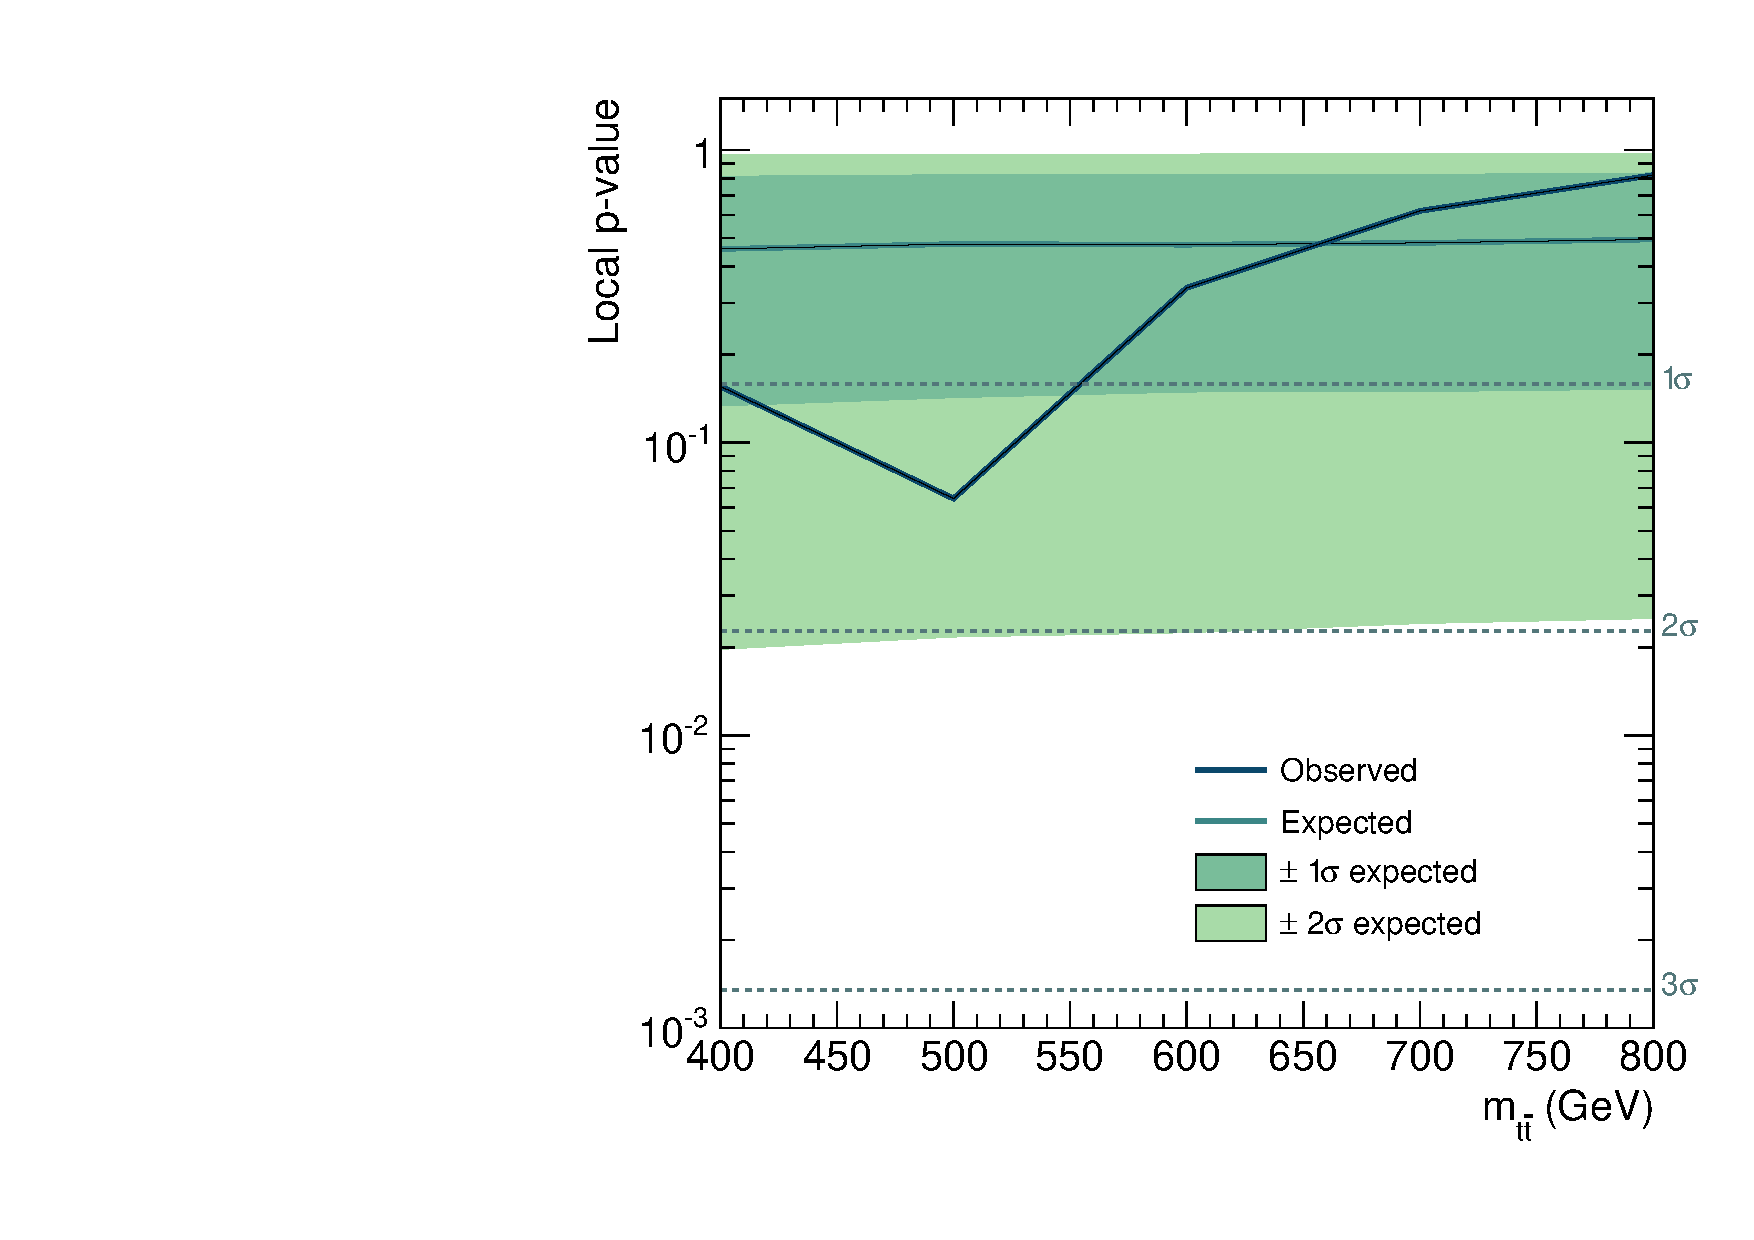
\includegraphics[width=0.65\textwidth,angle=-90,origin=c]{chapitre8/figs/pvalues_scalar.pdf}} \\
    \subcaptionbox{\sz pseudo-scalaire}[0.65\textwidth]{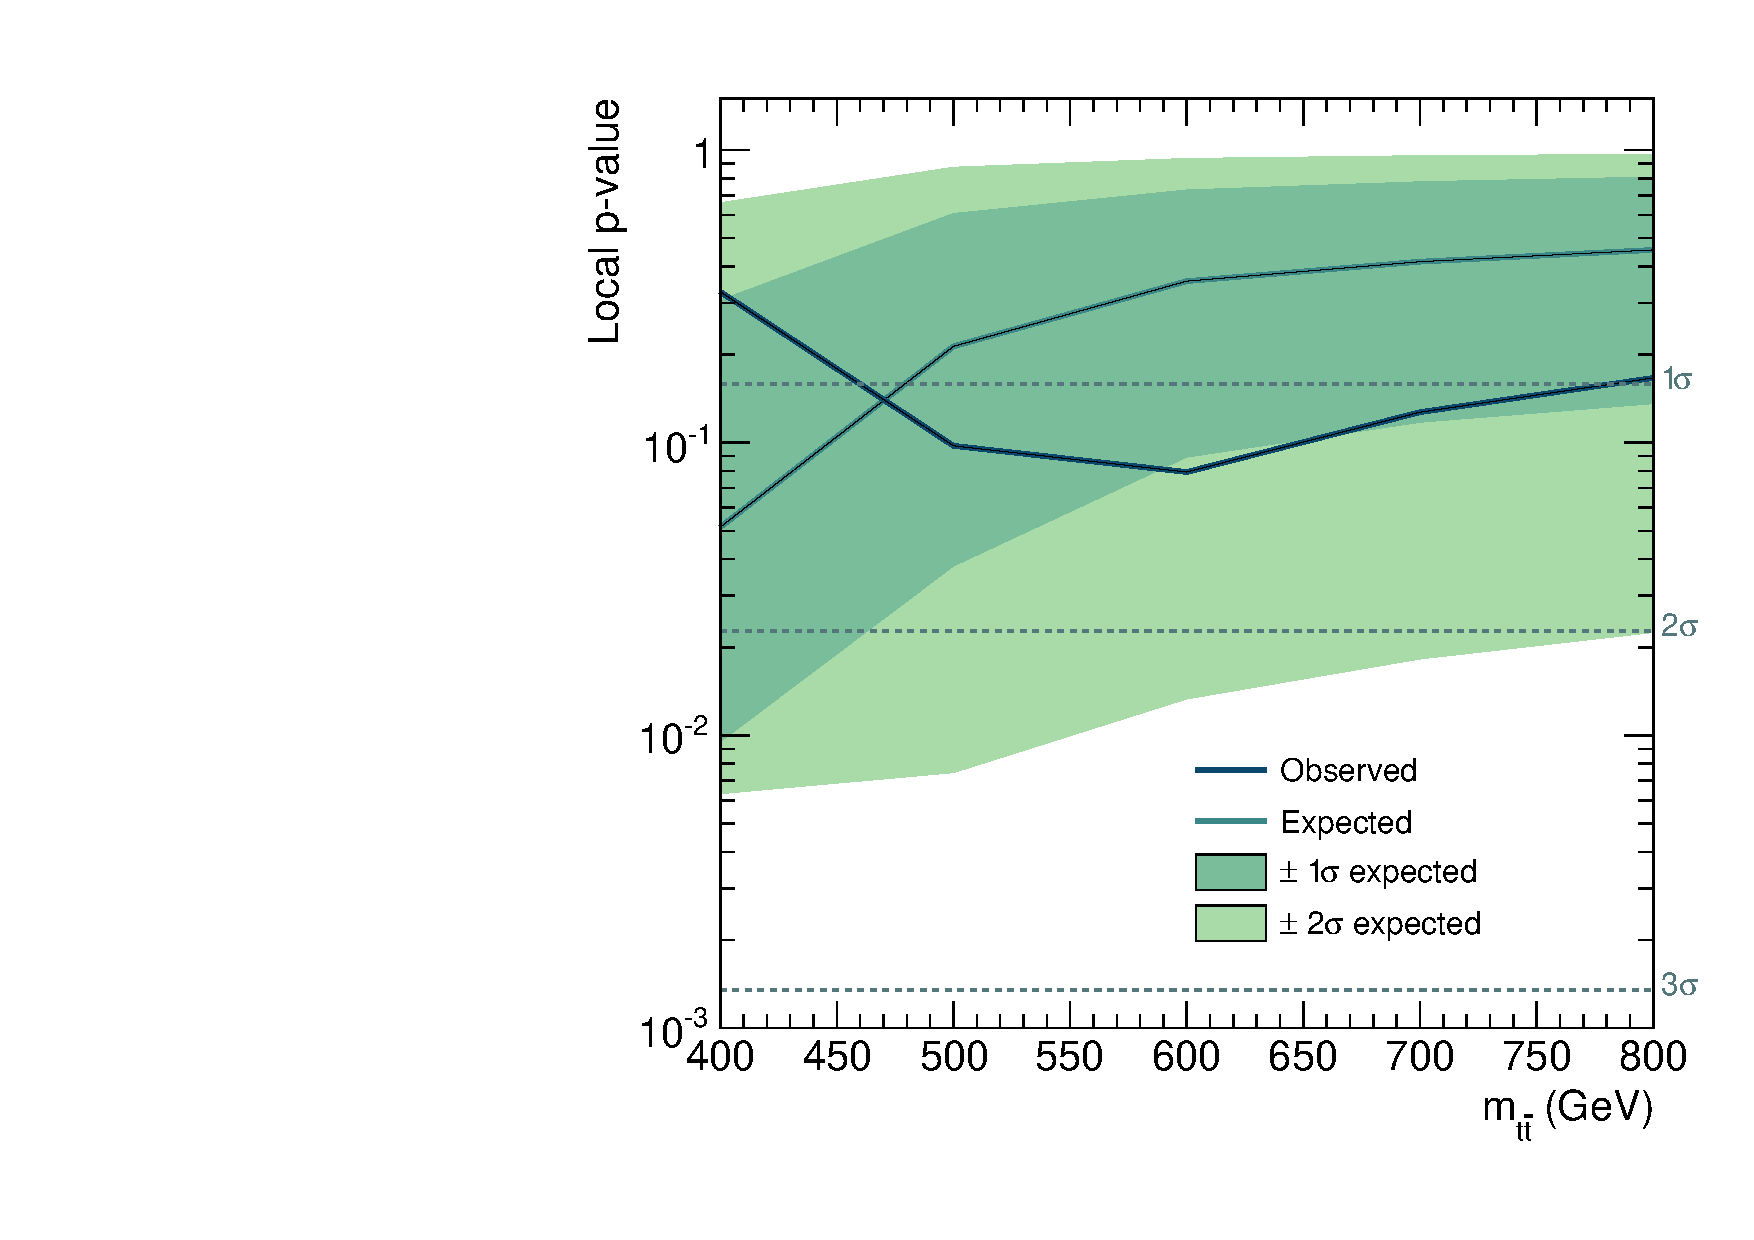
\includegraphics[width=0.65\textwidth,angle=-90,origin=c]{chapitre8/figs/pvalues_pseudoscalar.pdf}}
    \caption{Distributions des \pvalues pour chaque point de masse considérés. La ligne verte correspond aux \pvalues attendues et la ligne bleue aux \pvalues observées. Les bandes en vert foncé et vert clair correspondent respectivement aux intervalles de confiance à \SI{68}{\percent} et \SI{95}{\percent} sur la \pvalue attendue.}
    \label{fig:pvalues_mass}
\end{figure}

\section{Conclusion et perspectives}

Ce chapitre est consacré à la recherche de résonances scalaires et pseudo-scalaires dans le spectre de masse \ttbar, interférant avec la production de paires \ttbar du Modèle Standard. Une technique de génération a été développée spécifiquement pour cette analyse afin d'être en mesure de générer le signal accompagné des interférences.

\smallskip

La présence d'interférence modifie grandement la stratégie de l'analyse. Même si après reconstruction le déficit est atténué, il est néanmoins nécessaire de prendre en compte l'effet des interférences sur l'efficacité de sélection.

\bigskip

Finalement, la sensibilité de l'analyse n'est pas suffisante pour prétendre à une observation, une signification statistique d'au moins $3\sigma$ étant nécessaire. La meilleure signification statistique atteinte est d'environ \num{1.5}$\sigma$, pour un \sz pseudo\-/scalaire de basse masse. Il est ainsi nécessaire d'améliorer l'analyse afin d'être sensible à un signal de nouvelle physique. Plusieurs pistes peuvent être explorées :
\begin{itemize}
    \item Il est nécessaire d'éviter au maximum le recouvrement entre les partie positives et négatives du signal reconstruit, ce qui permet d'augmenter l'efficacité de la sélection, et ainsi la sensibilité de l'analyse. Pour cela, la piste de l'ajustement cinématique semble la plus prometteuse. Même si les tests effectués lors des précédentes études (voir \cref{sec:mtt_kf,sec:zprime_kf}) n'ont pas été concluants, l'algorithme peut être configuré de plusieurs manières différentes (contraintes, résolutions, ...), qui n'ont pas toutes été testées.

    \item L'analyse présentée dans ce chapitre est complètement dépendante du modèle de nouvelle physique considéré. Ainsi, il est possible d'ajouter des coupures exploitant les différences topologiques entre les événements de nouvelle physique et les événements du Modèle Standard.
\end{itemize}

\begin{table} \centering
\begin{tabular}{ccccc} \toprule
 & \multicolumn{2}{c}{$\sigma_\text{scalaire}$} & \multicolumn{2}{c}{$\sigma_\text{pseudo-scalaire}$} \\ \cmidrule{2-5}
 & \SI{400}{\GeV} & \SI{800}{\GeV} & \SI{400}{\GeV} & \SI{800}{\GeV} \\ \midrule
 \SI{8}{\TeV} & \SI{0,5289}{\pb} & \SI{0,0944}{\pb} & \SI{1,169}{\pb} & \SI{0,2325}{\pb} \\
 \SI{14}{\TeV} & \SI{1.767}{\pb} & \SI{0.3616}{\pb} & \SI{3.757}{\pb} & \SI{0.8296}{\pb} \\ \cmidrule{1-1}
 Gain & $\times\,\num{3,34}$ & $\times\,\num{3,83}$ & $\times\,\num{3,21}$ & $\times\,\num{3,57}$ \\
 \bottomrule
\end{tabular}
\caption{Comparaison entre les sections efficaces à l'arbre à \SI{8}{\TeV} et \SI{14}{\TeV} prédites par \texttt{MadGraph} pour un \sz de masse $\msz = \SI{400}{\GeV}$ ou $\msz = \SI{800}{\GeV}$. La dernière ligne présente le gain de la montée en énergie, à comparer au facteur \num{3,9} d'augmentation de la section efficace \ttbar Modèle Standard.}
\label{tab:sigma_14tev}
\end{table}

Lors du redémarrage du LHC à \SI{14}{\TeV}, les sections efficaces de production vont augmenter. Les gains attendus pour différentes masses sont résumés dans le \cref{tab:sigma_14tev}. Ces gains sont à comparer au facteur \num{3,9} d'augmentation de la section efficace \ttbar Modèle Standard à \SI{14}{\TeV}.

Comme discuté précédemment, il n'est pas évident d'évaluer les changements dans la distribution de masse invariante simplement à partir de ces valeurs. Une estimation préliminaire est toutefois possible en utilisant les distributions obtenues à \SI{8}{\TeV} et les sections efficaces à \SI{14}{\TeV}. Dans cette hypothèse et pour une luminosité collectée de \SI{100}{\invfb}, le gain en signification statistique le plus important est obtenu pour un pseudo\-/ scalaire de masse $\msz = \SI{400}{\GeV}$, pour lequel une signification statistique de 2\sigma{} est atteinte.

\end{fmffile}